\subsubsection{Instructions}
This guide describes the steps required to solder and assemble HestiaPi Touch ONE
from parts.  Assembly with the case and wall is covered in Section
\ref{Wall Installation ONE}.

\begin{enumerate}
  \item Solder standard headers onto PCB for the pi (figure \ref{fig:pi_headers})
	  Make sure you don't miss the reset pin at the right, just below the
		block of 2x20 pins
  \item Solder the pi onto those headers (figure \ref{fig:pi})
  \item Put terminal block and sendor headers in place and solder them on (figures
	  \ref{fig:terminal_block_in_place} and \ref{fig:terminal_block_soldered})
  \item Solder relays in place (figure \ref{fig:relays})
  \item Solder the headers onto the BME board (figures \ref{fig:BME} and
	  \ref{fig:BME_soldered})
  \item Solder switch in place (figure \ref{fig:switch})
  \item Pull the long headers so the top of the pin is 12mm off of the board,
	  do this for all of the pins in the LCD headers
	  (figures \ref{fig:header} and \ref{fig:headers})
  \item Solder the LCD headers into place and connect the BME280 board
	  (\ref{fig:fully_assembled})
  \item If using the AC/DC converter, solder that on
\end{enumerate}

\begin{figure}
  \centering
  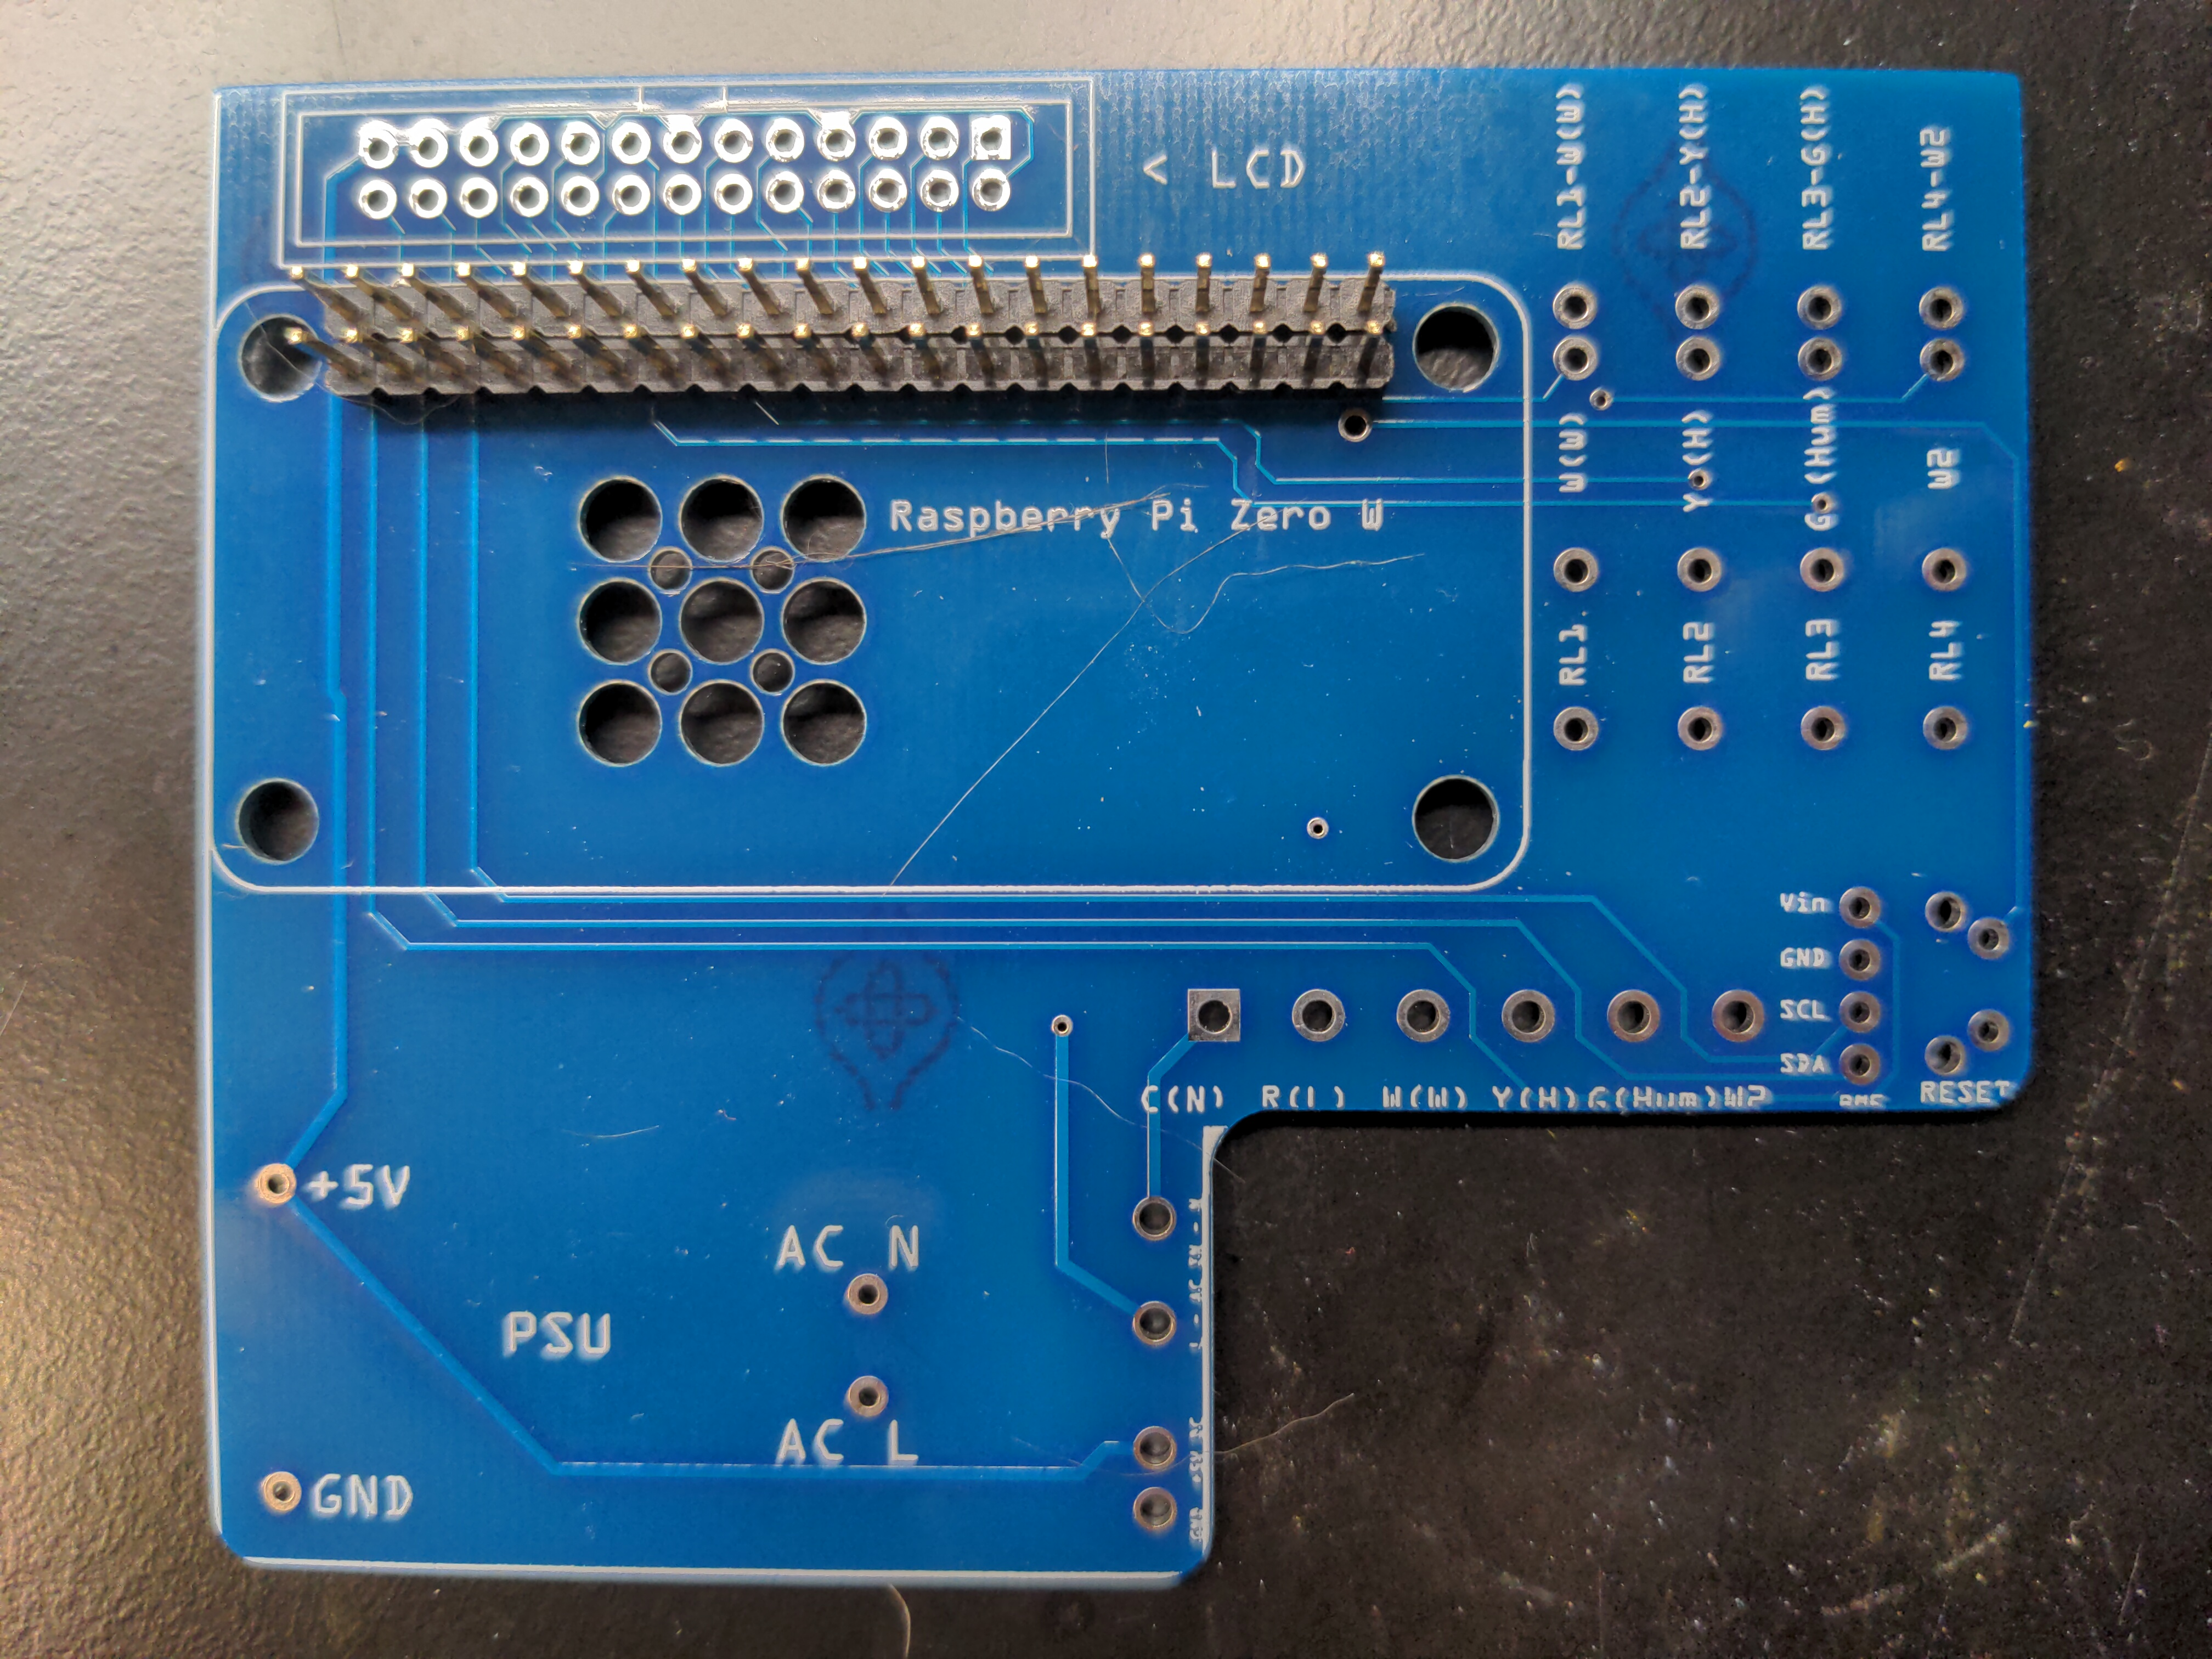
\includegraphics[width=3in]{img/pi_header_placement_soldered_on.jpg}
  \caption{Headers for the pi, don't forget the reset pin like I did here!}
  \label{fig:pi_headers}
\end{figure}
\begin{figure}
  \centering
  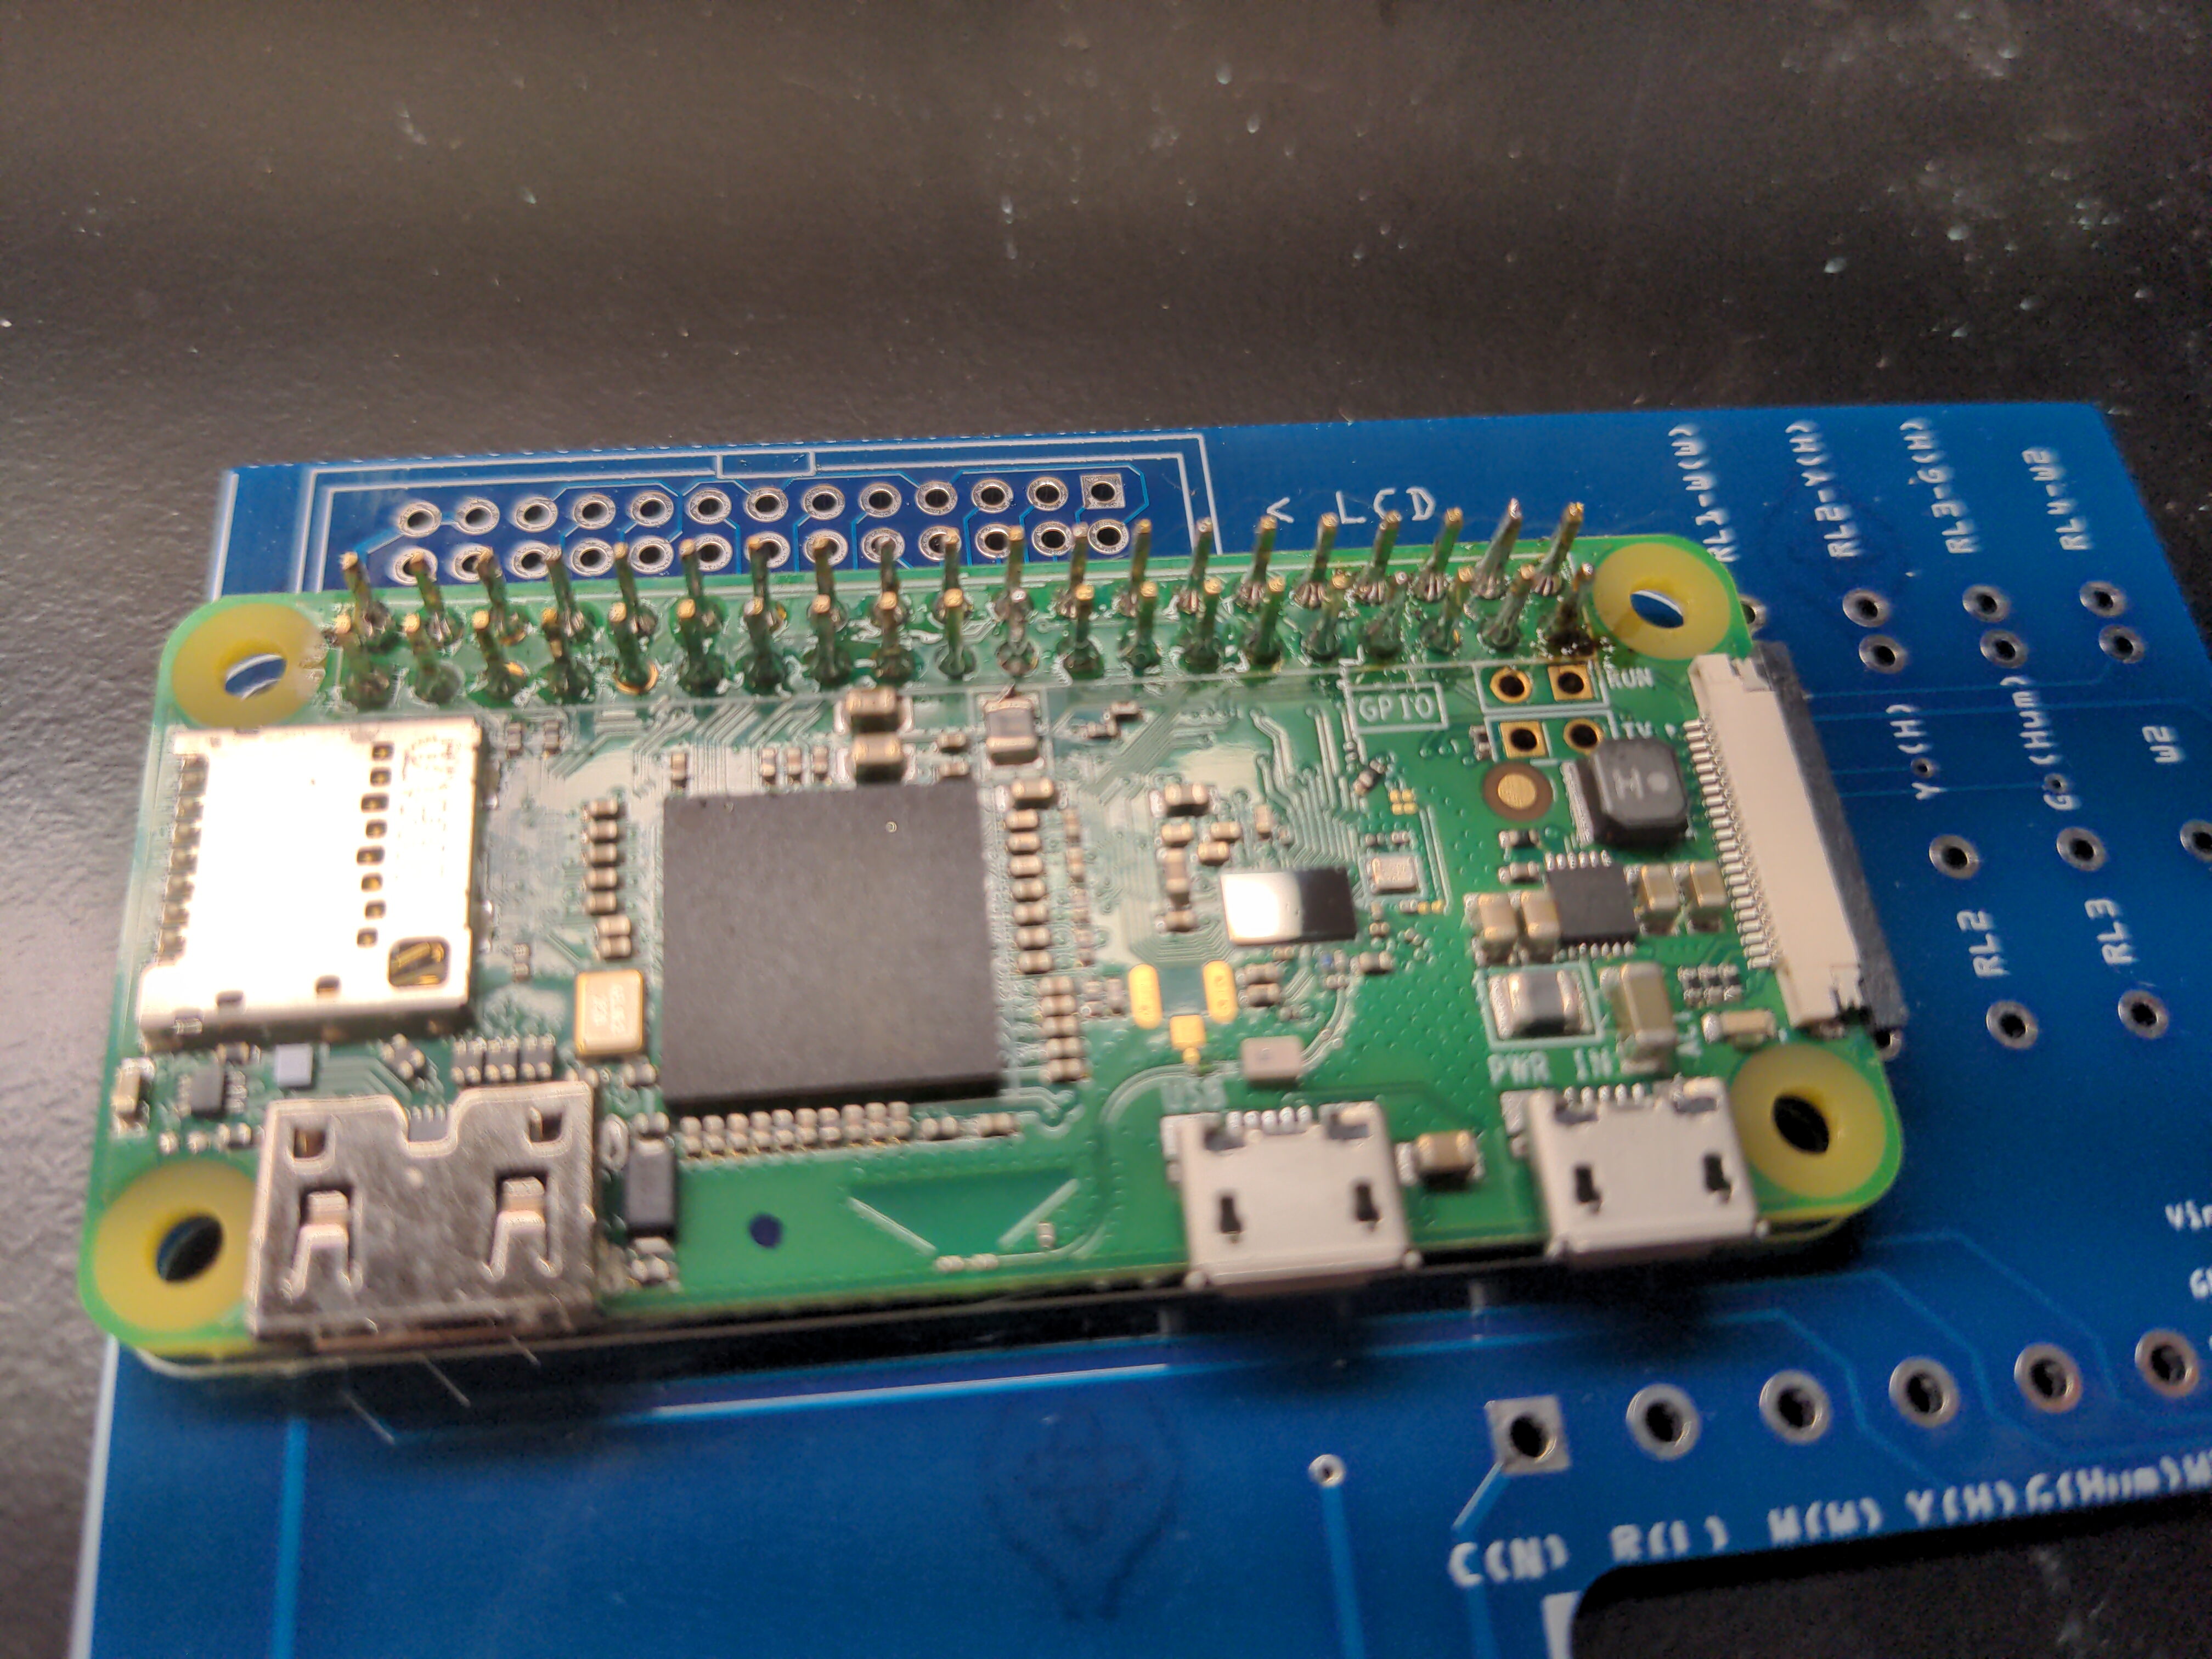
\includegraphics[width=3in]{img/pi_soldered_on.jpg}
  \caption{Pi soldered on, sans the reset pin that I had to go back and patch
	up later}
  \label{fig:pi}
\end{figure}
\begin{figure}
  \centering
  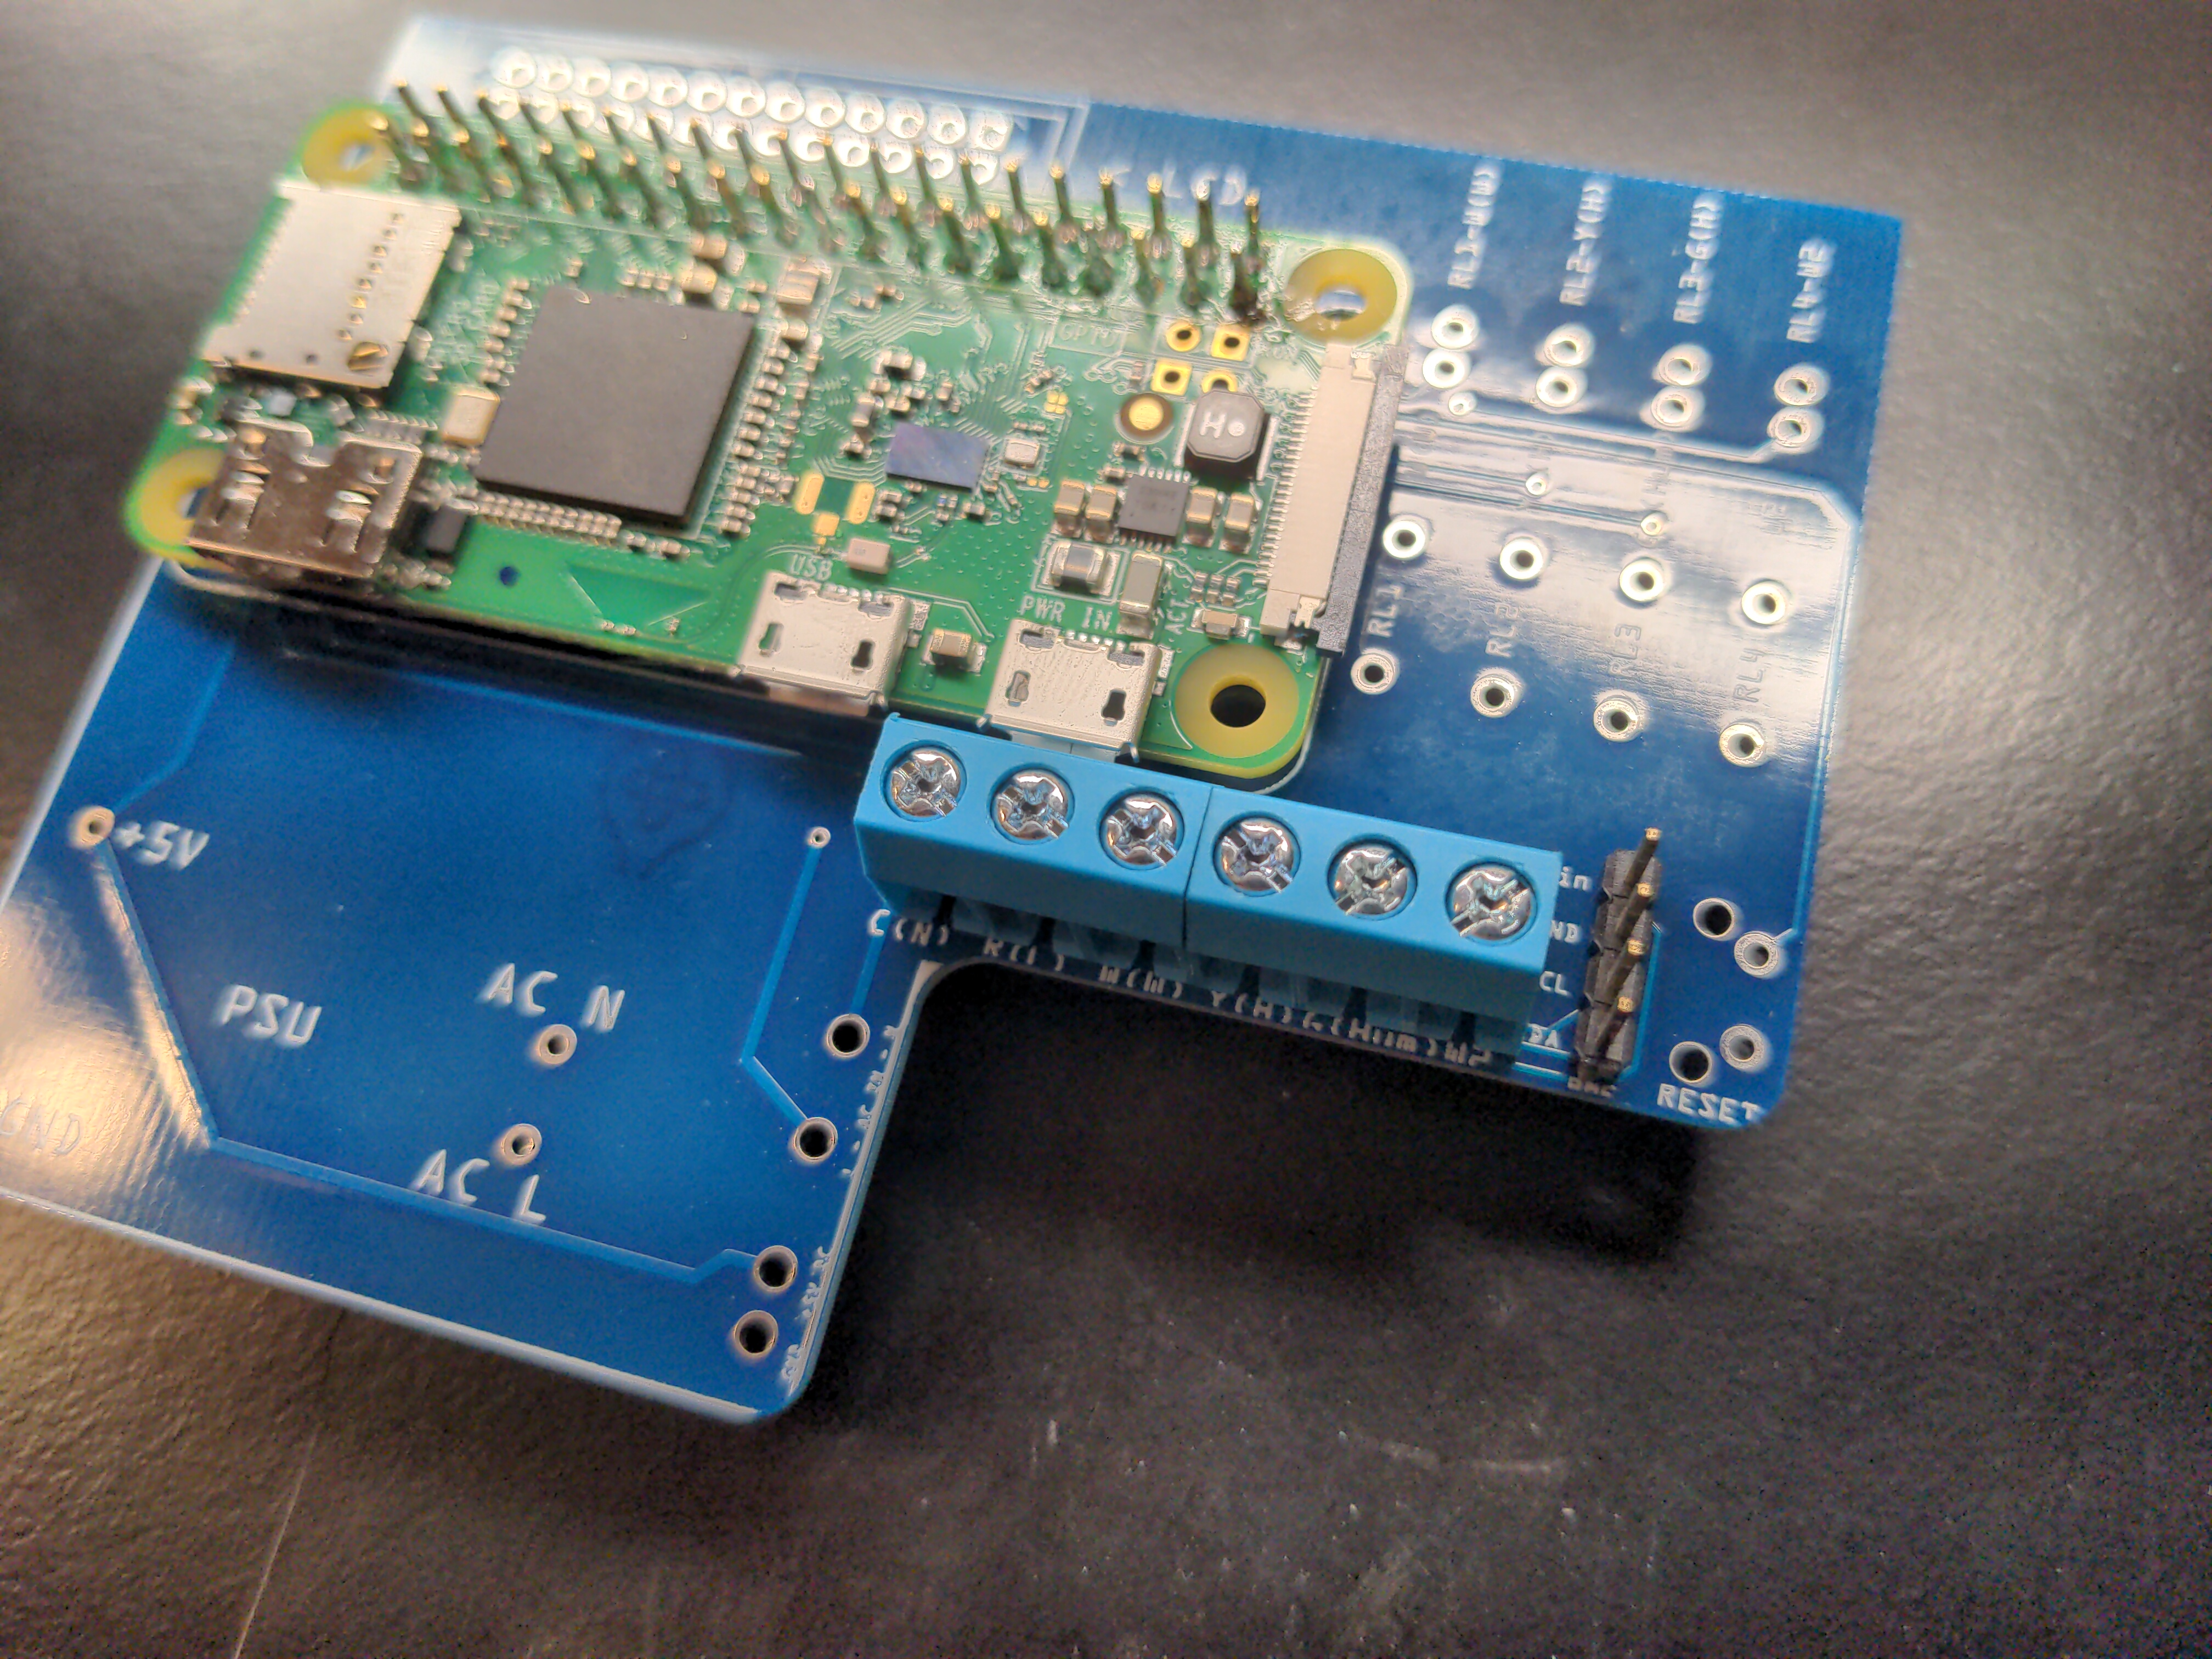
\includegraphics[width=3in]{img/terminal_block_placement.jpg}
  \caption{Terminal block and sensor headers in place}
  \label{fig:terminal_block_in_place}
\end{figure}
\begin{figure}
  \centering
  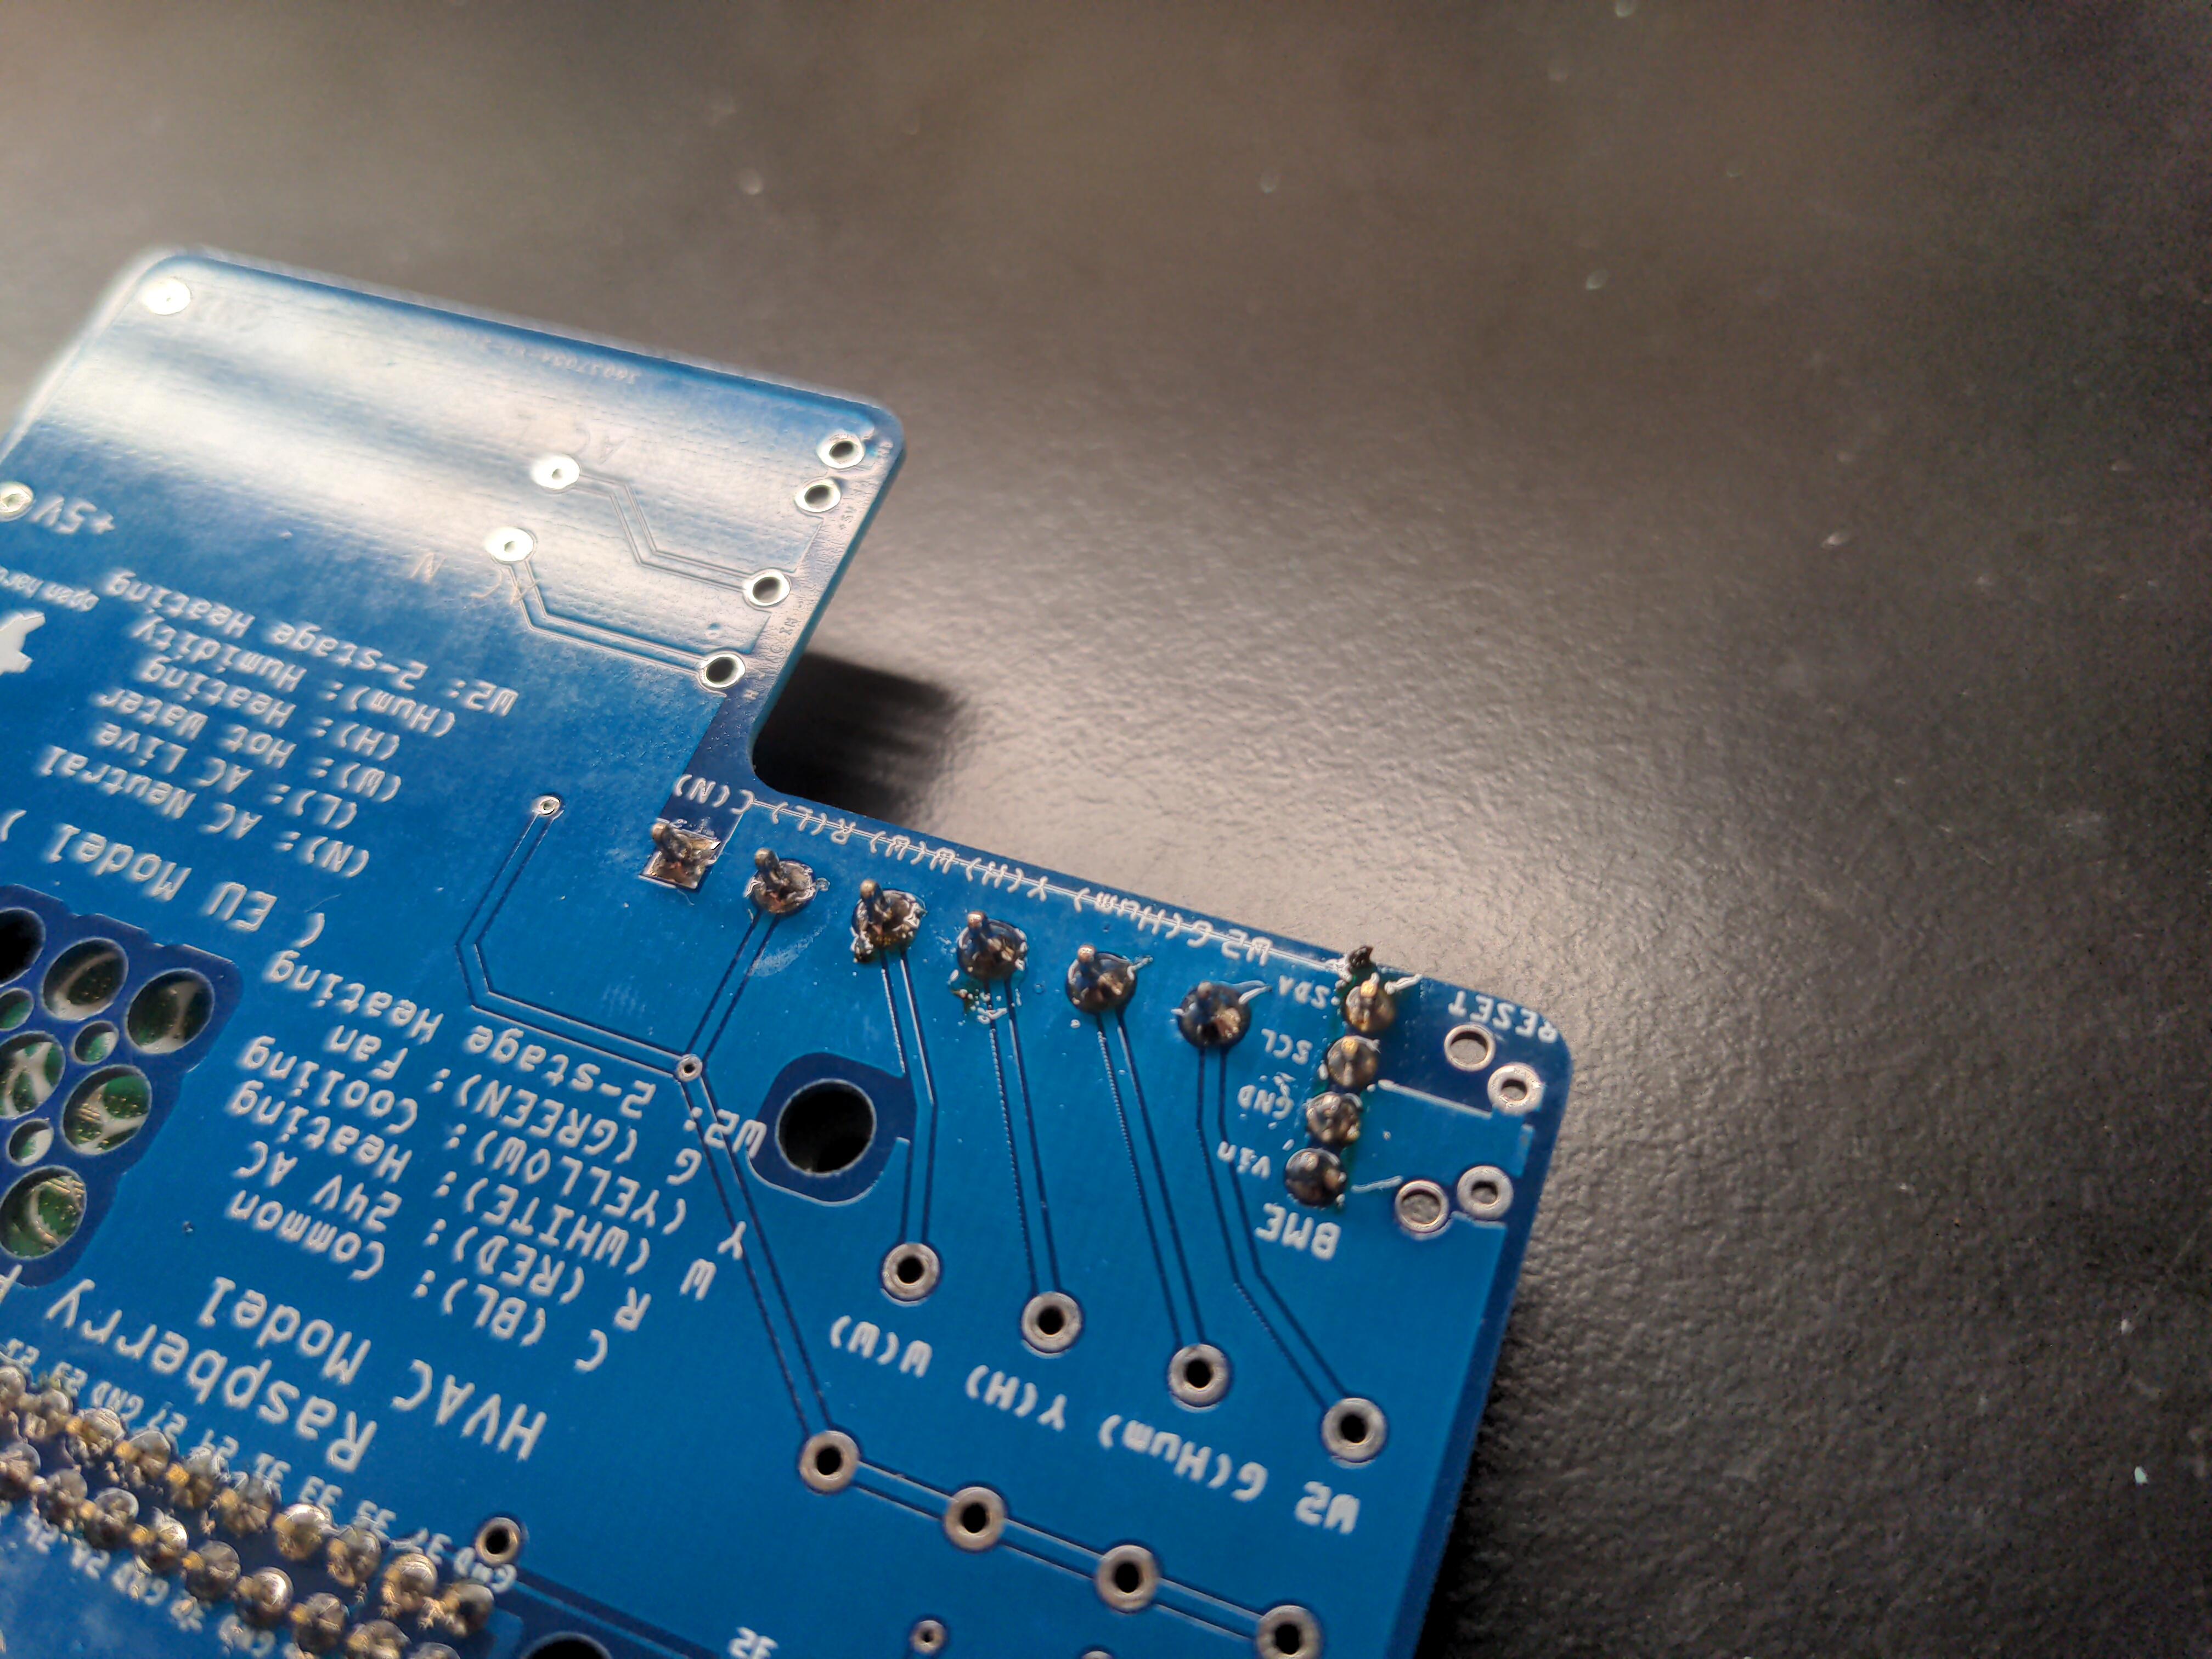
\includegraphics[width=3in]{img/terminal_block_soldered.jpg}
  \caption{Terminal block and sensor headers soldered on}
  \label{fig:terminal_block_soldered}
\end{figure}
\begin{figure}
  \centering
  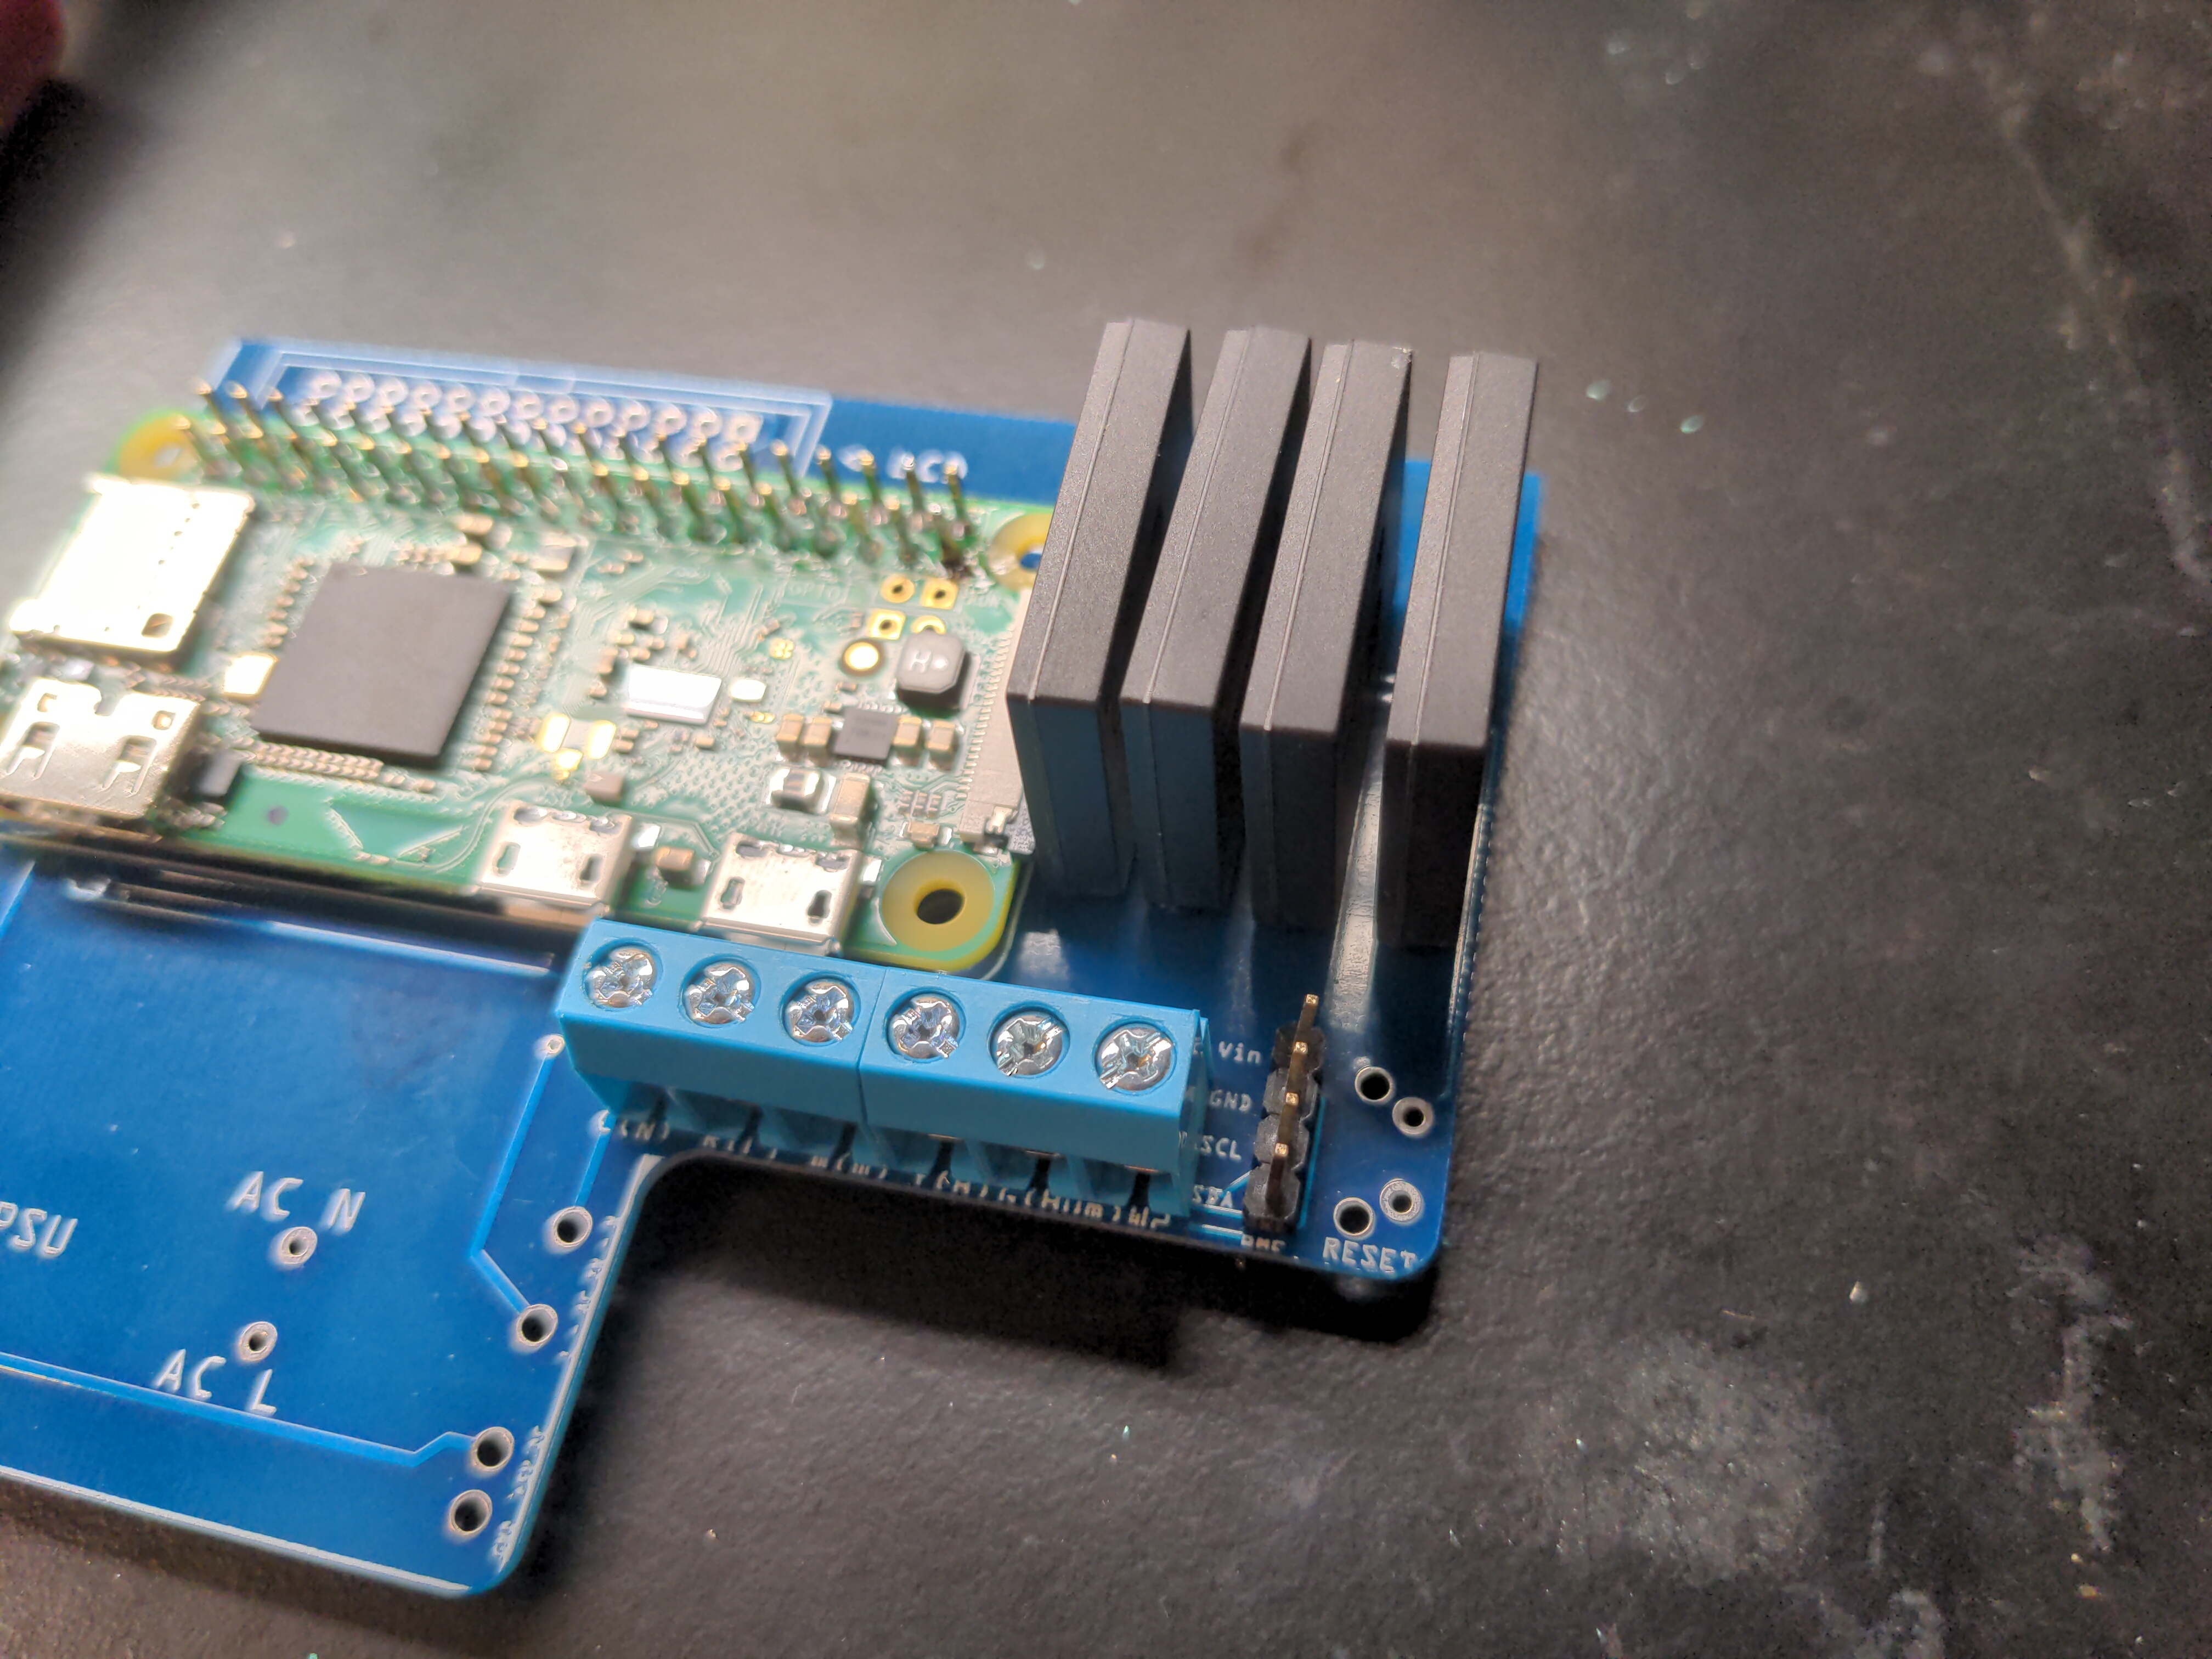
\includegraphics[width=3in]{img/relay_placement.jpg}
  \caption{Relays soldered into place}
  \label{fig:relays}
\end{figure}
\begin{figure}
  \centering
  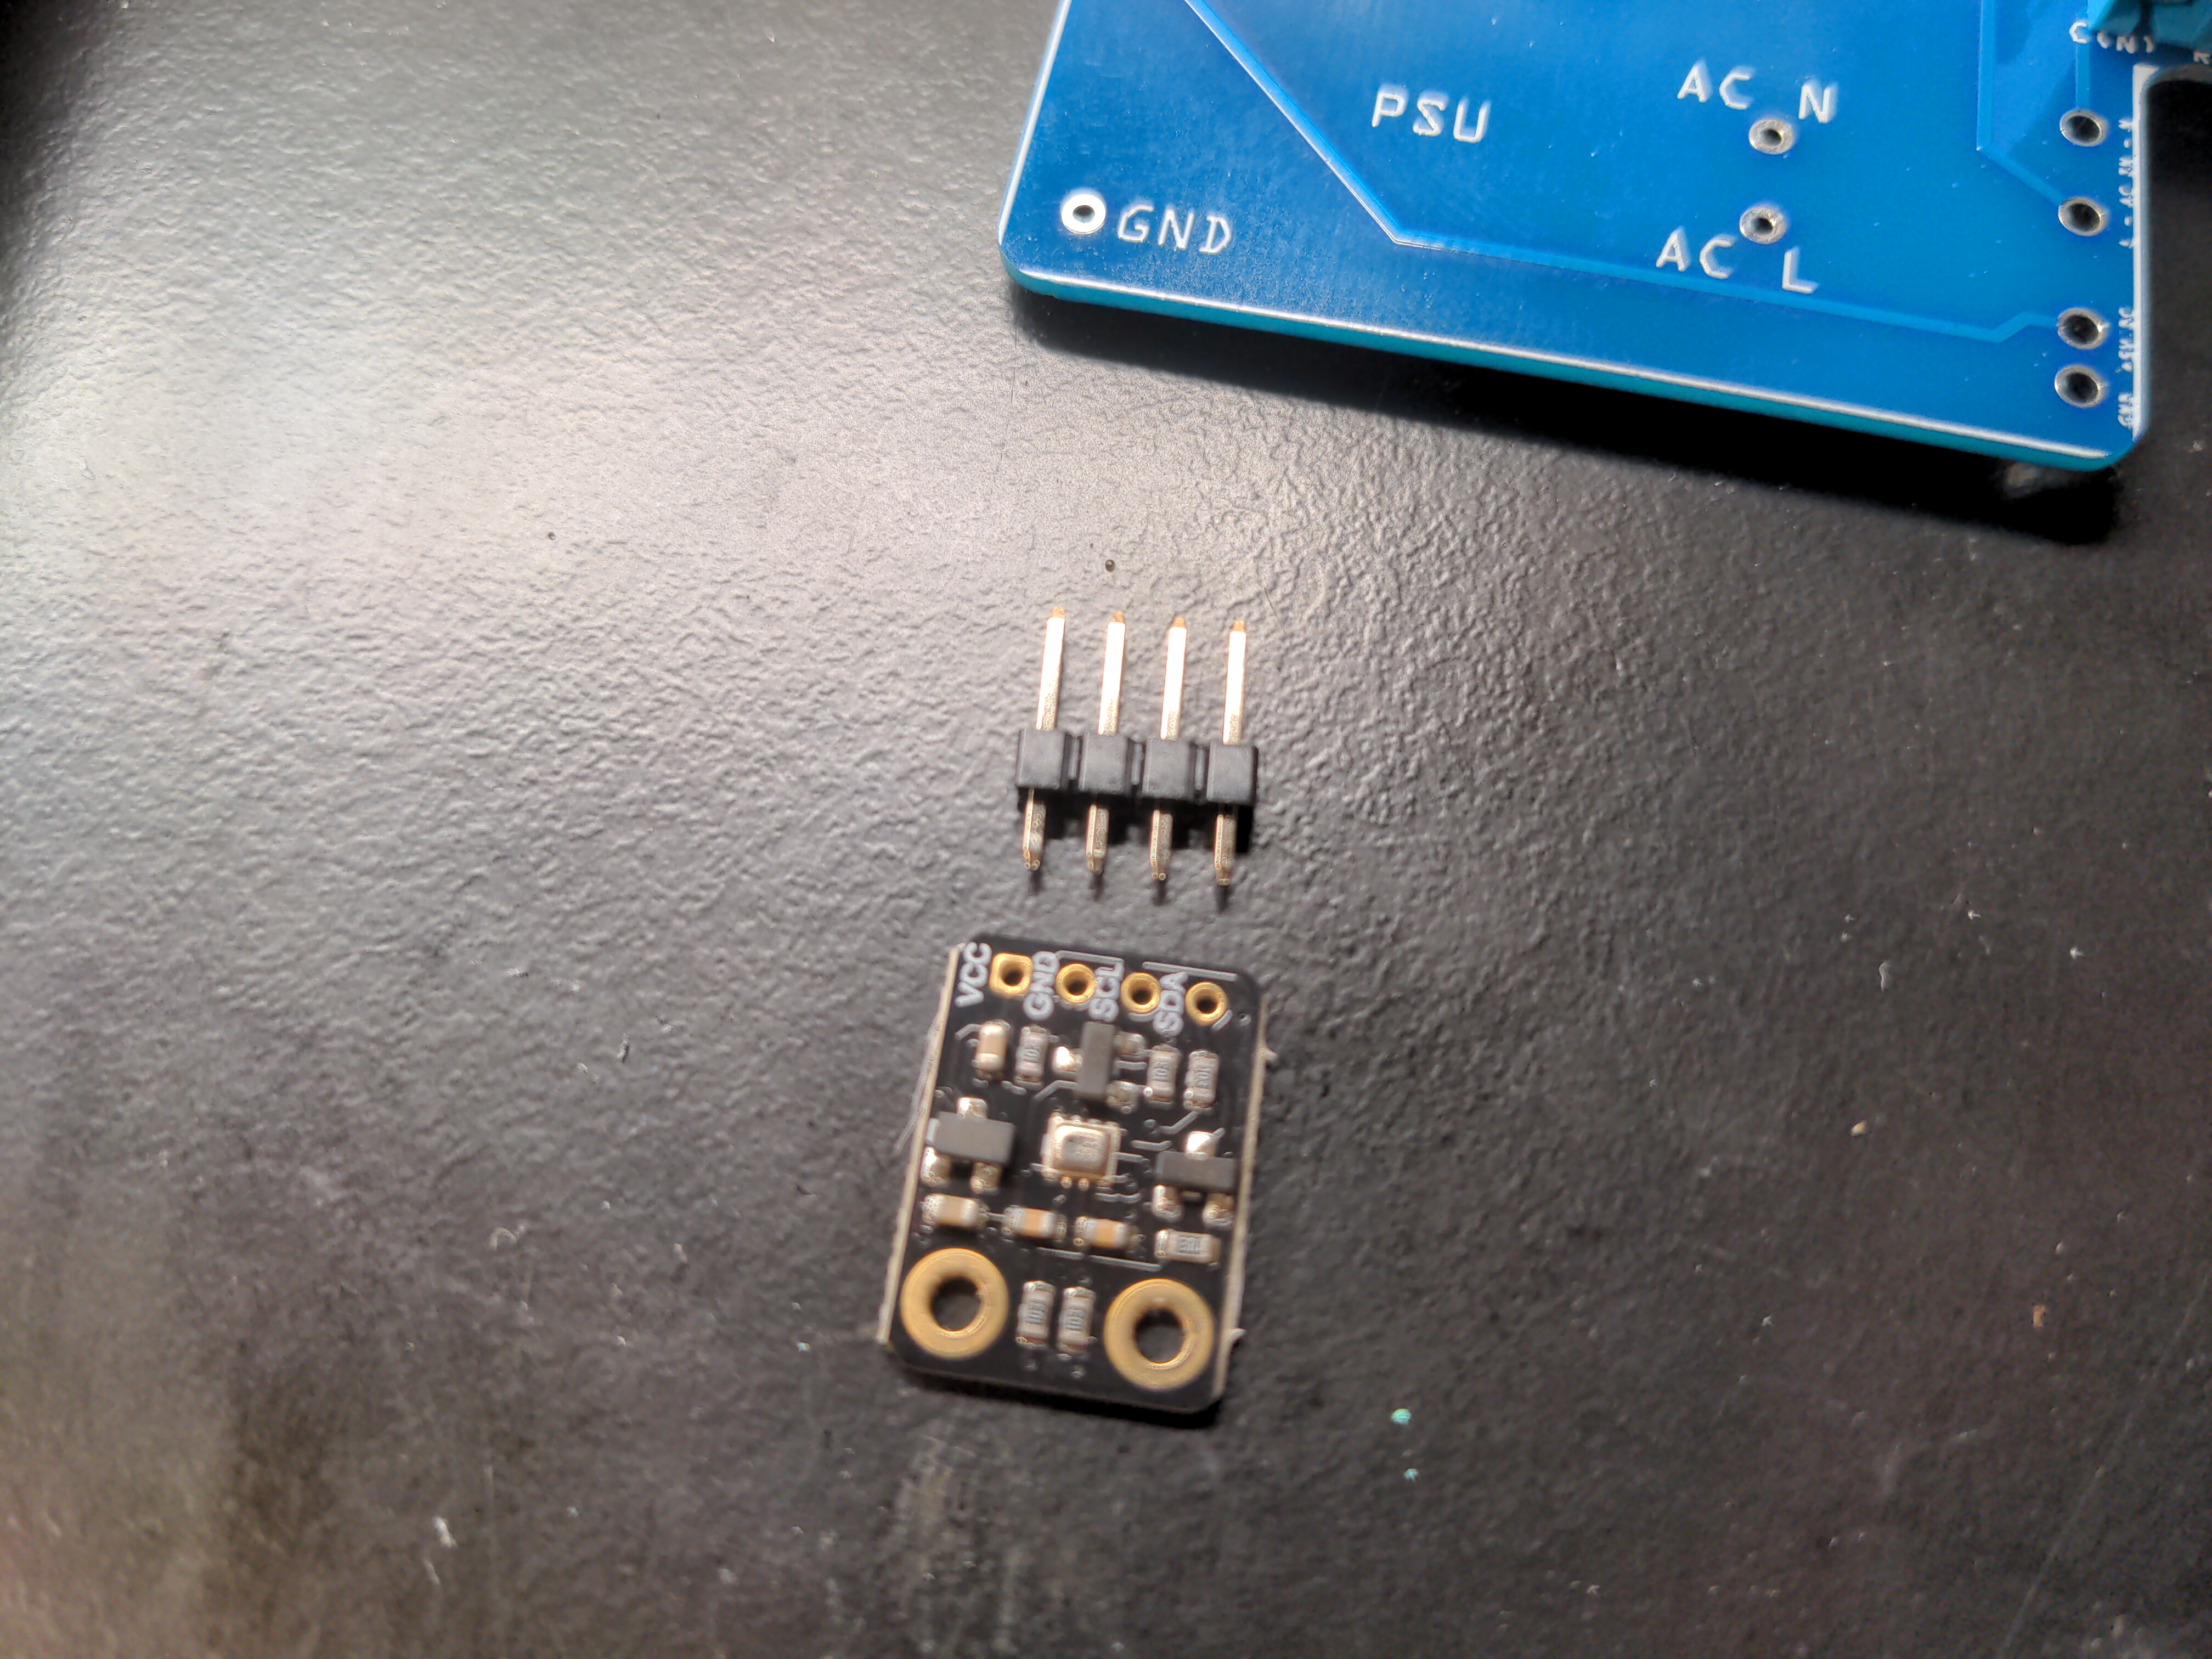
\includegraphics[width=3in]{img/BME280.jpg}
  \caption{BME needs to have headers attached}
  \label{fig:BME}
\end{figure}
\begin{figure}
  \centering
  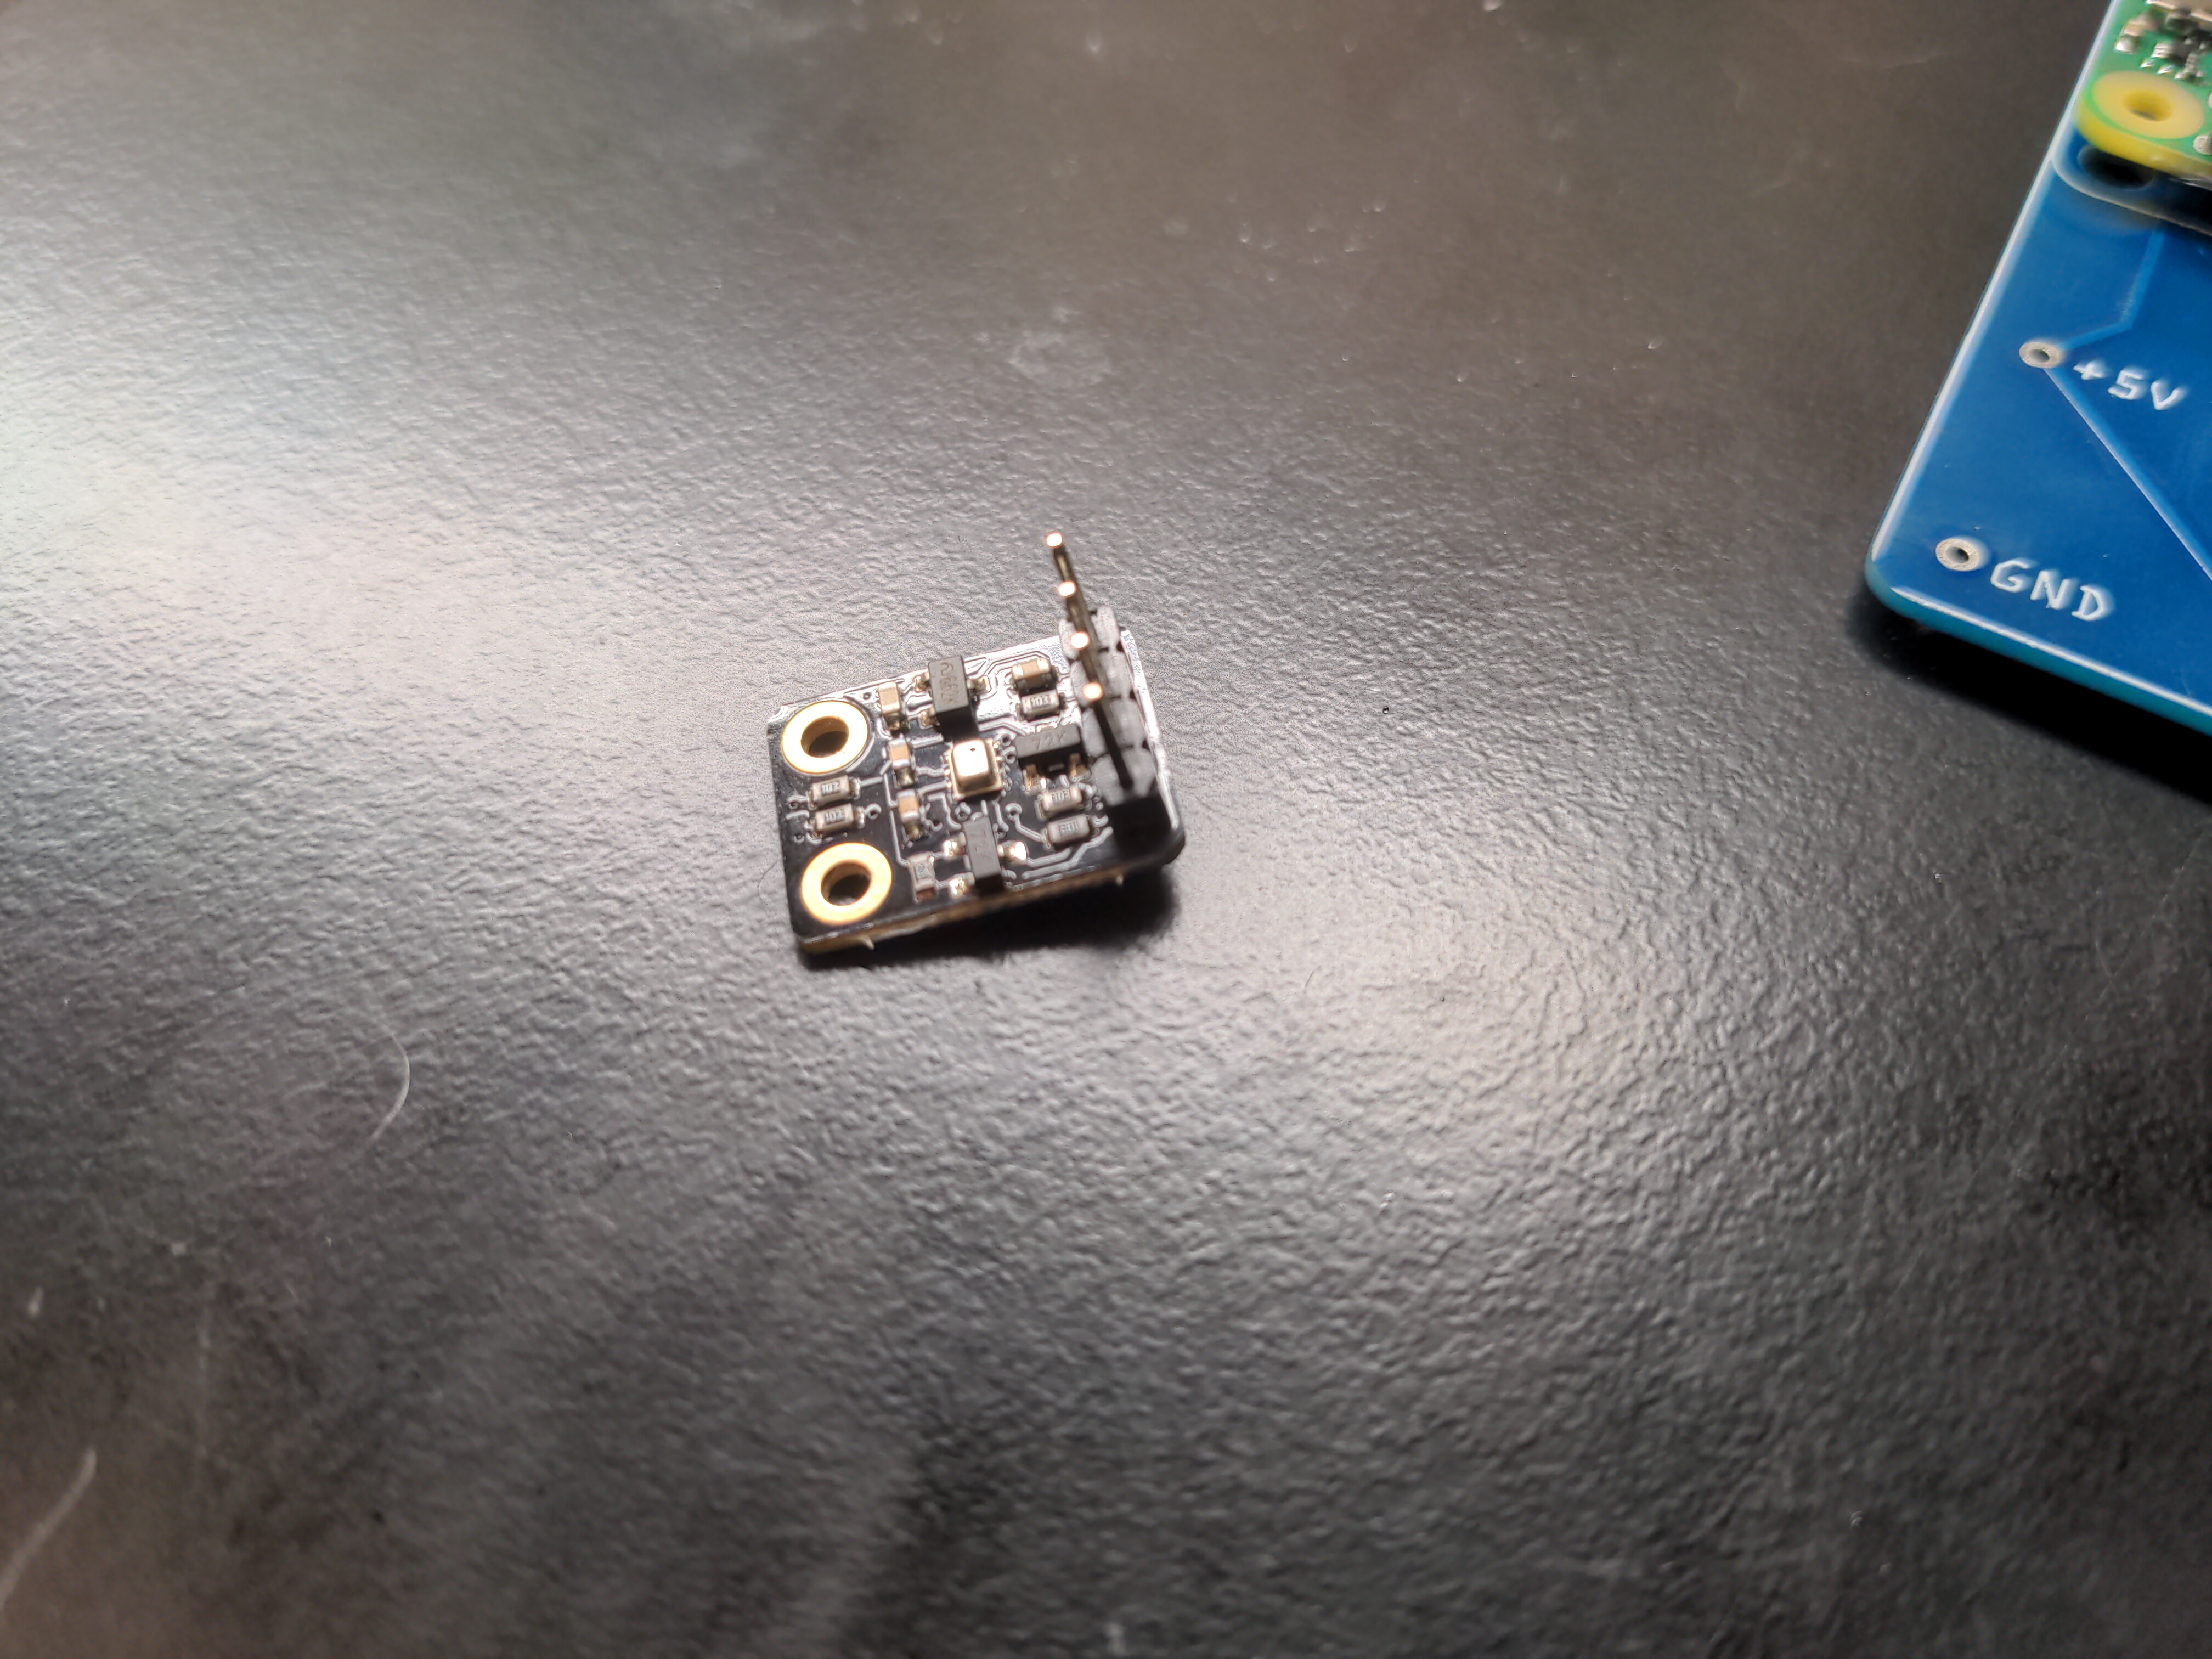
\includegraphics[width=3in]{img/BME280_assembled.jpg}
  \caption{BME with headers soldered on}
  \label{fig:BME_soldered}
\end{figure}
\begin{figure}
  \centering
  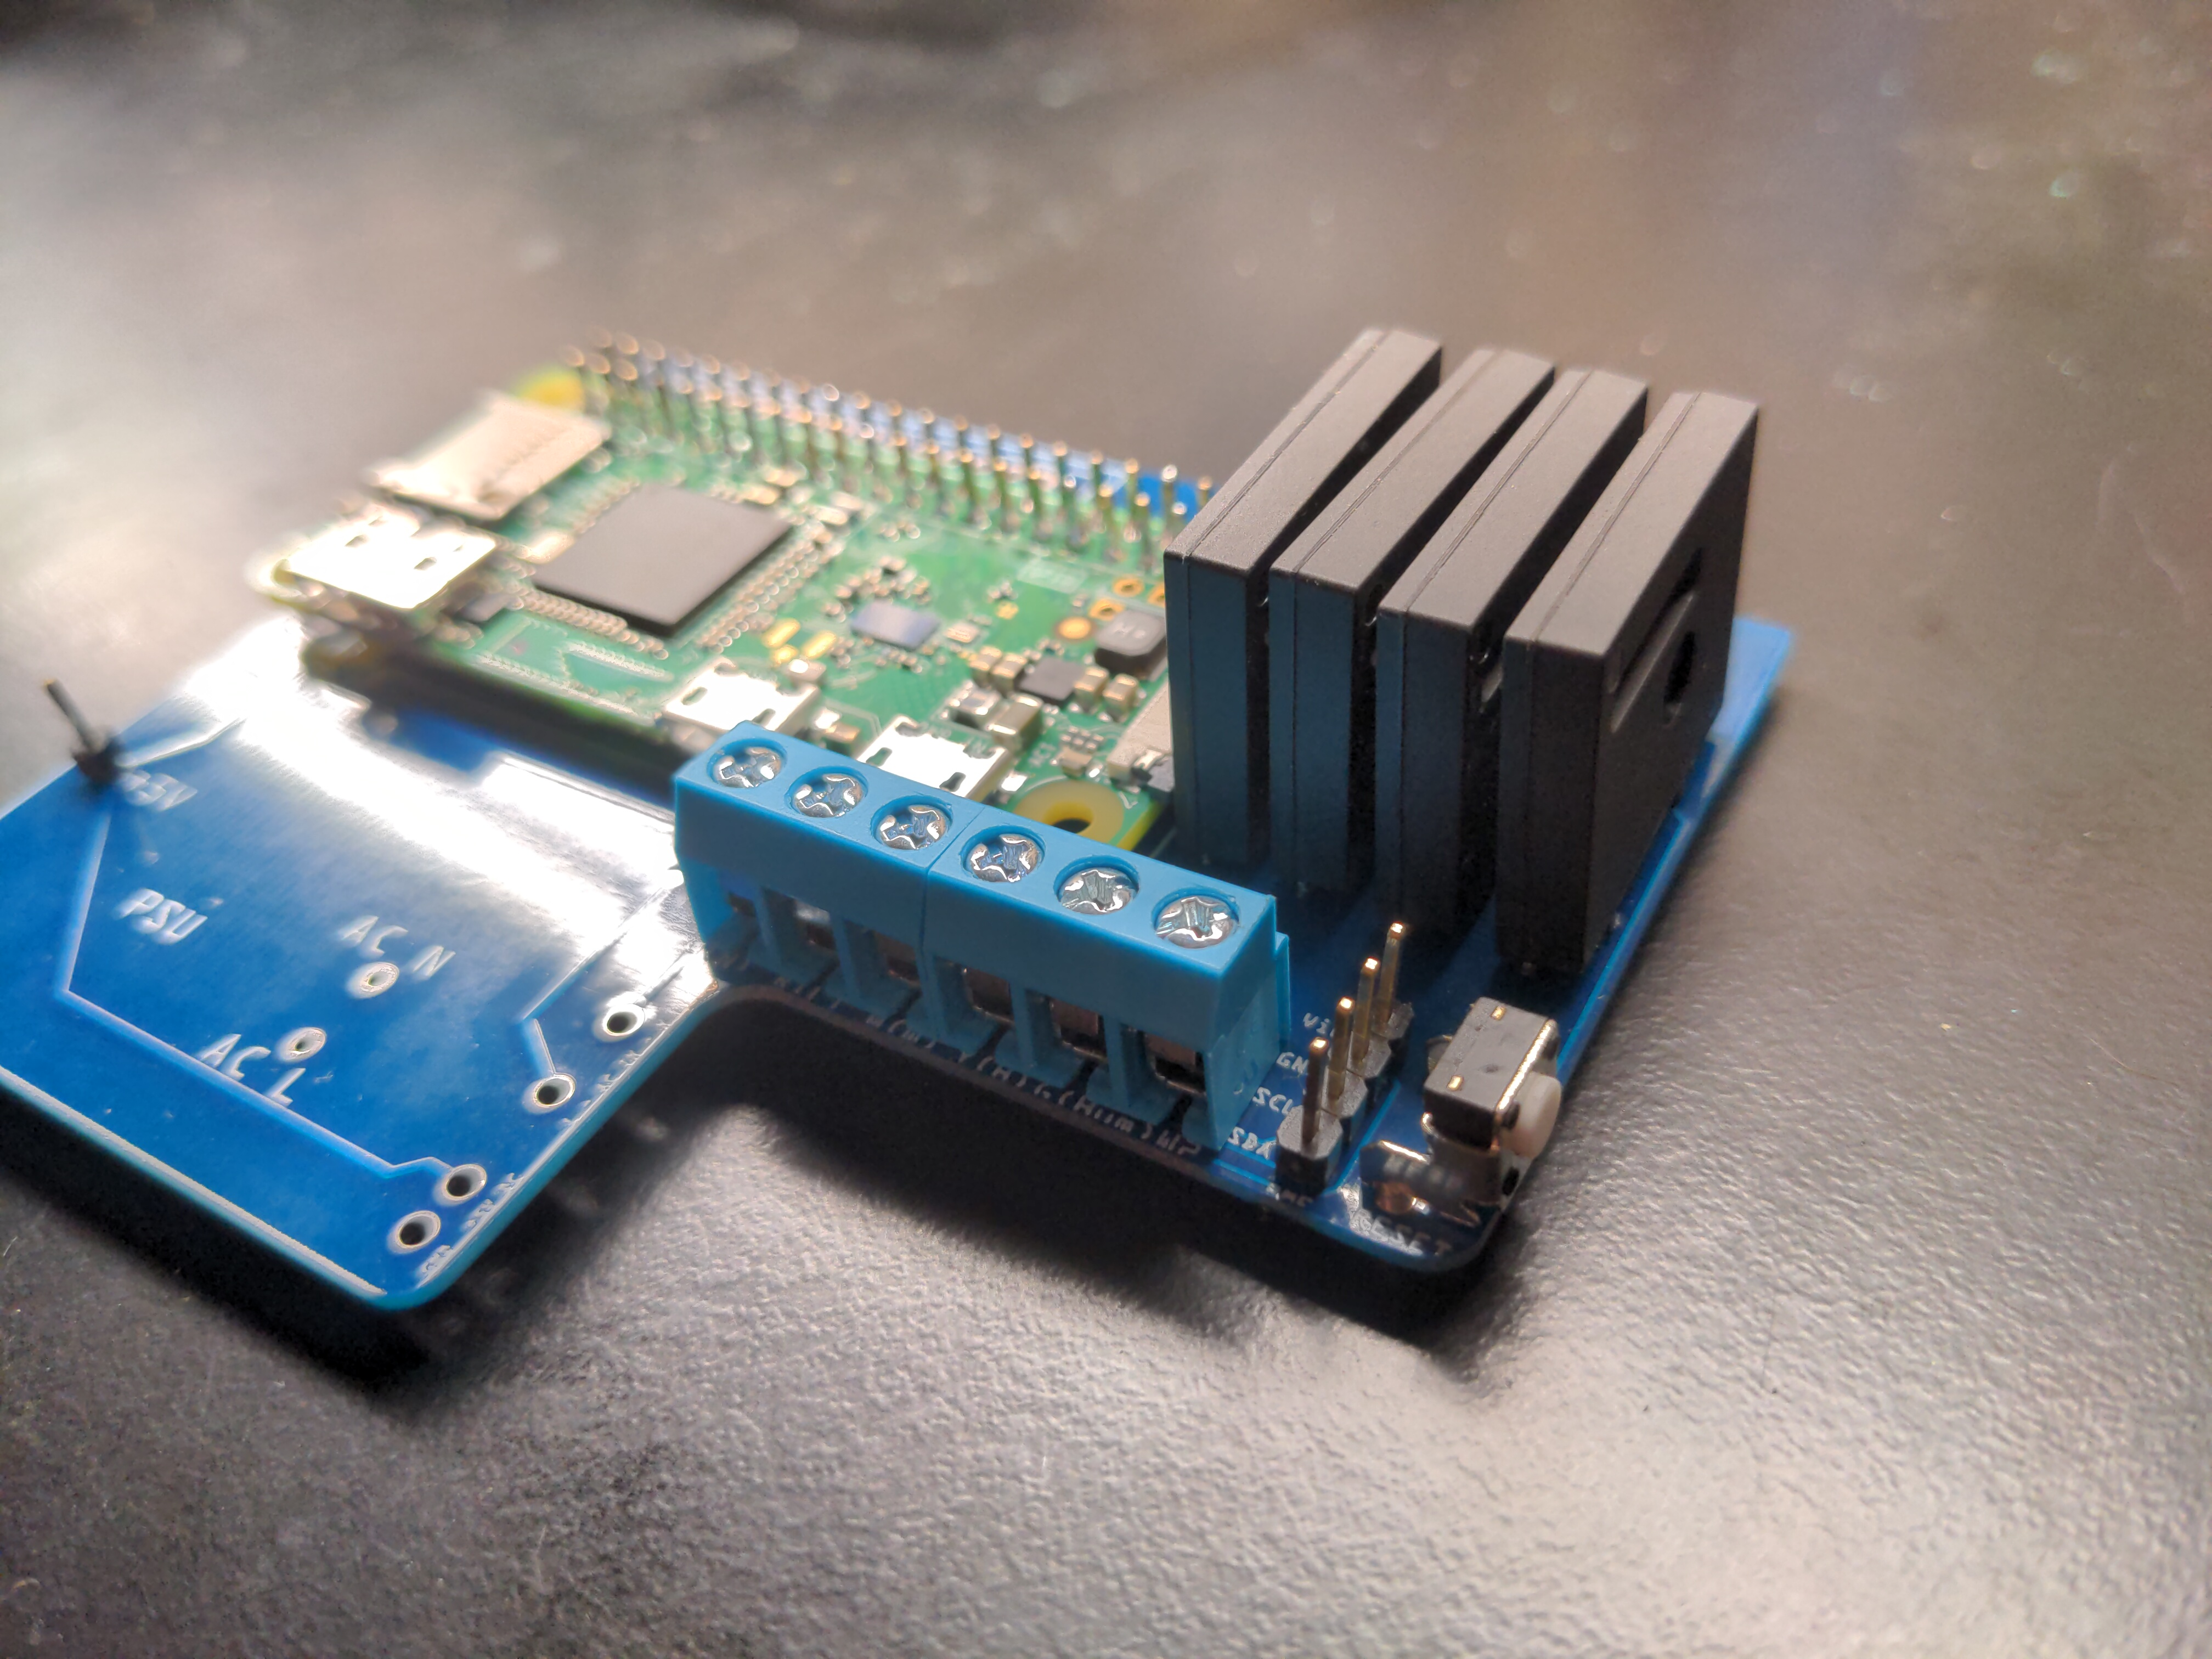
\includegraphics[width=3in]{img/switch.jpg}
  \caption{Solder switch into place}
  \label{fig:switch}
\end{figure}
\begin{figure}
  \centering
  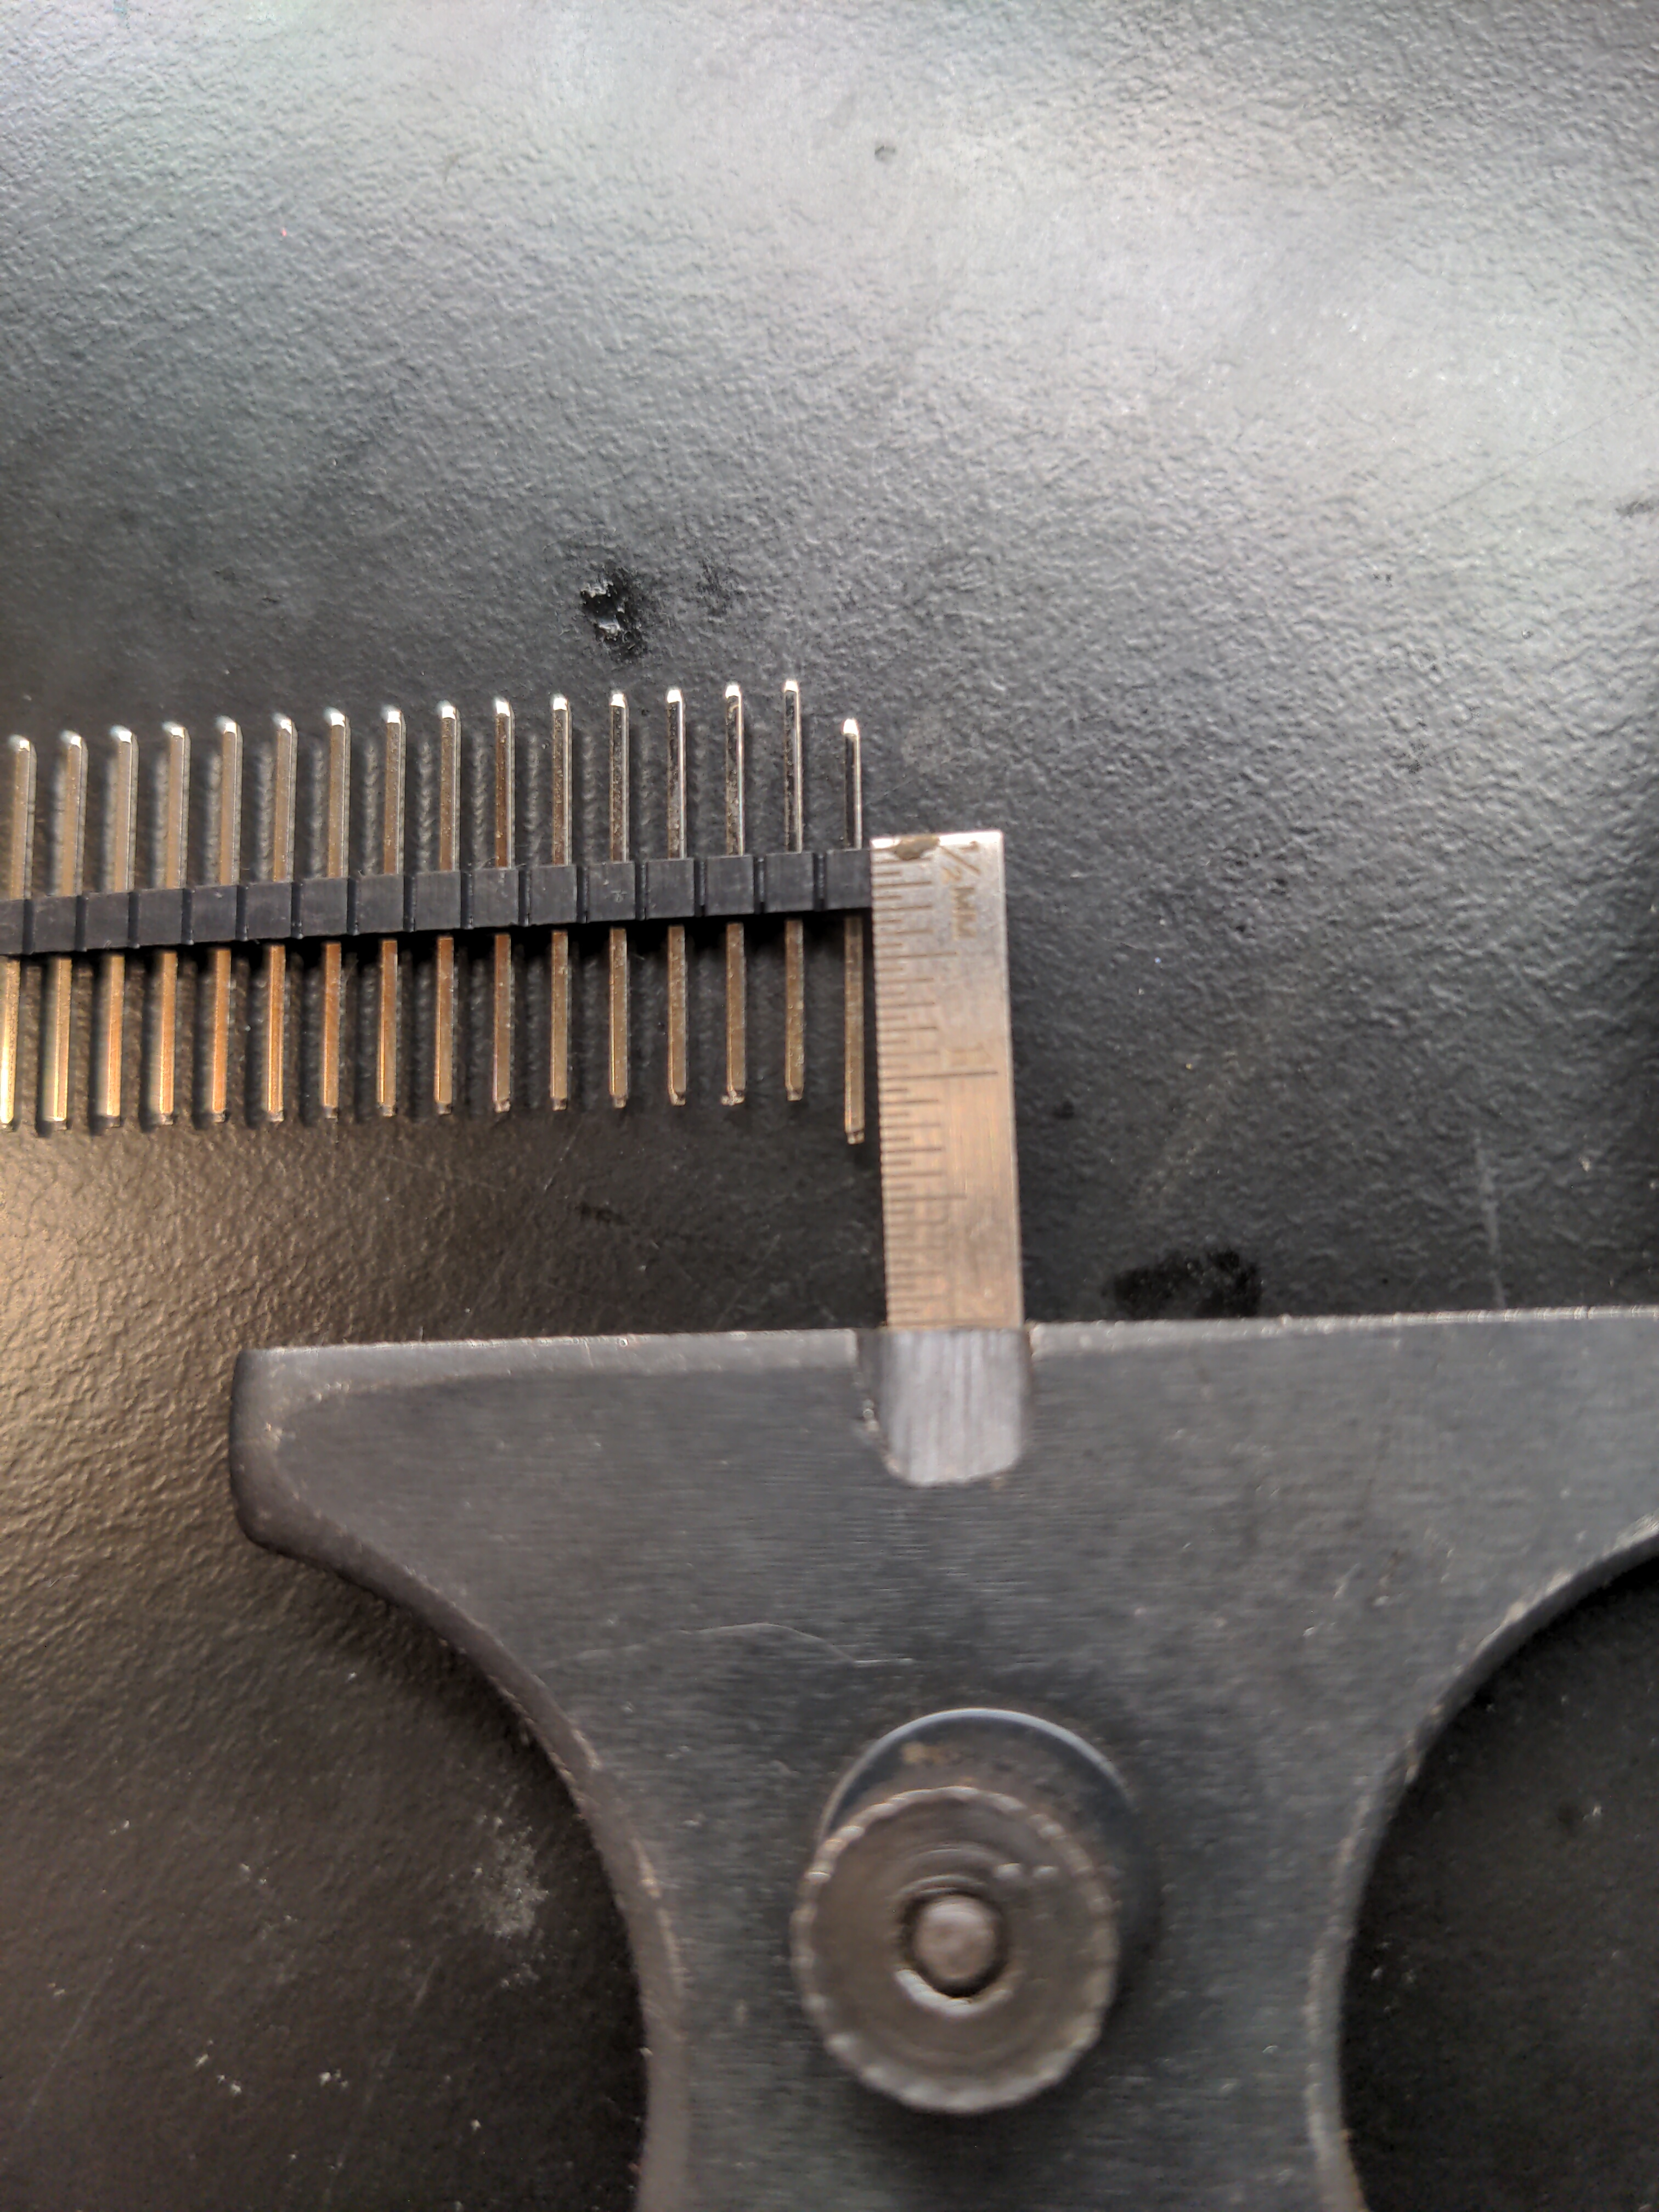
\includegraphics[width=3in]{img/modified_header.jpg}
  \caption{Pin placement adjusted to have 12mm above the board}
  \label{fig:header}
\end{figure}
\begin{figure}
  \centering
  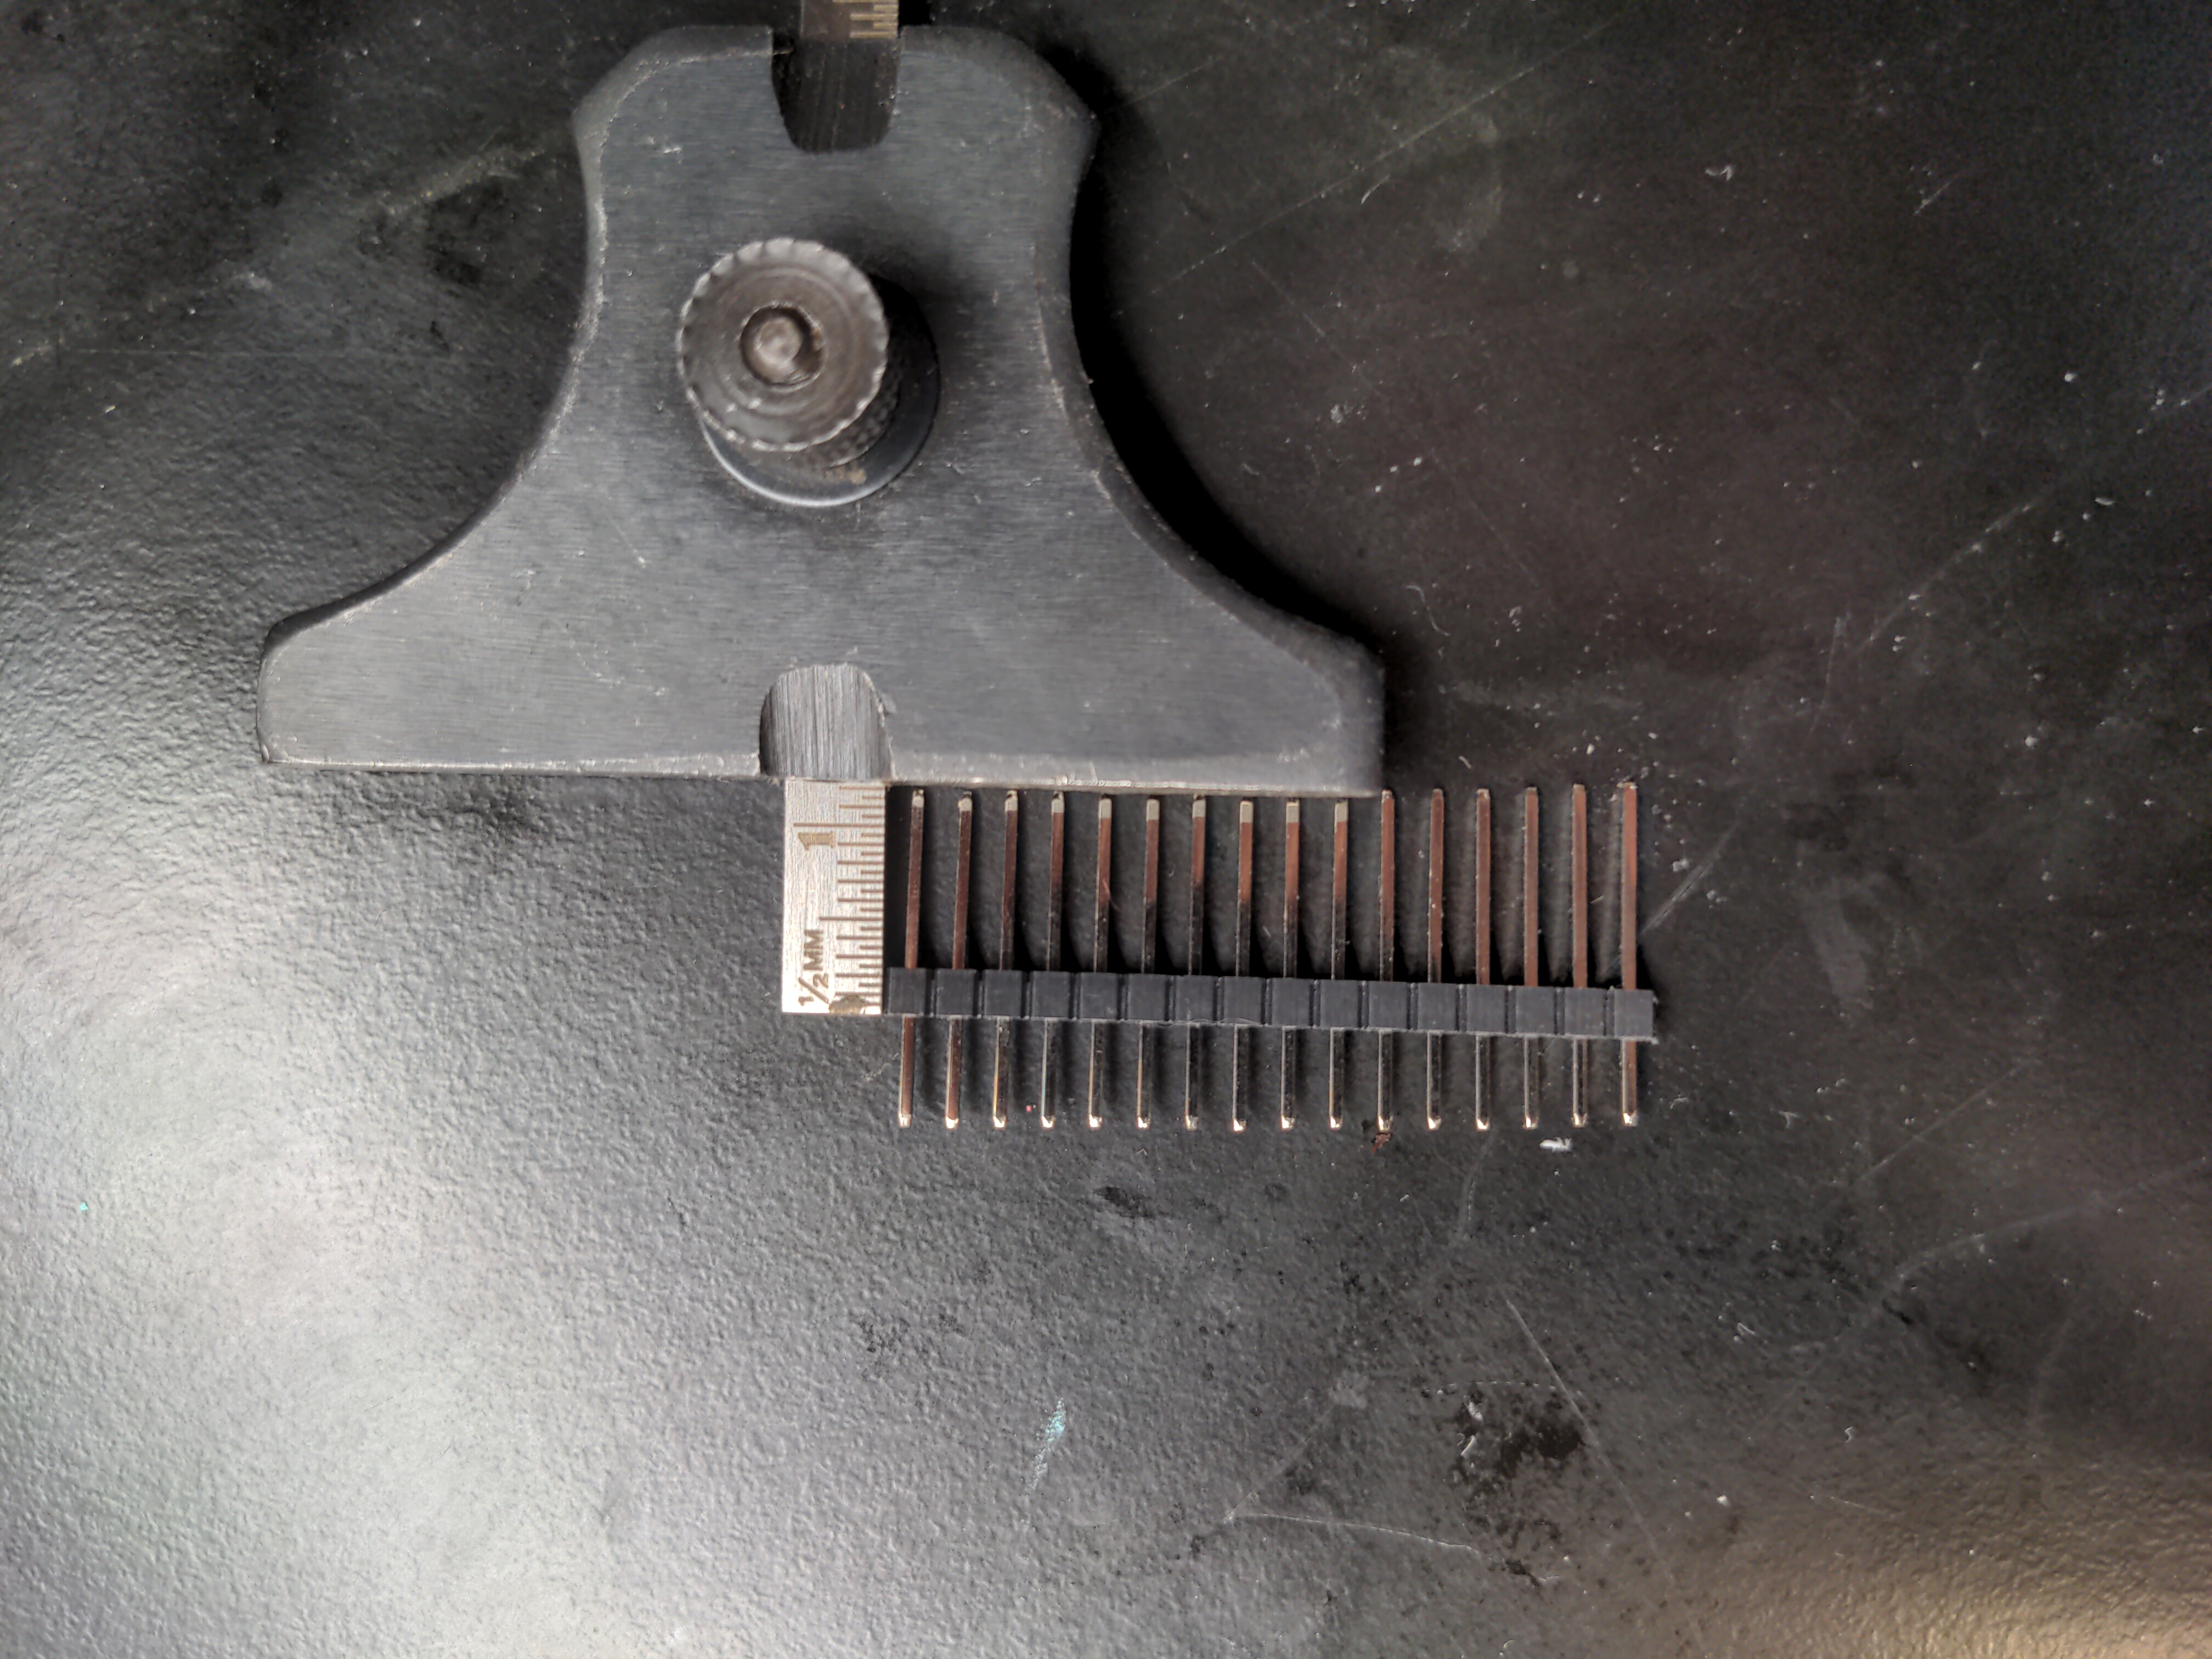
\includegraphics[width=3in]{img/modified_headers.jpg}
  \caption{All headers adjusted to be 12mm above the board}
  \label{fig:headers}
\end{figure}
\begin{figure}
  \centering
  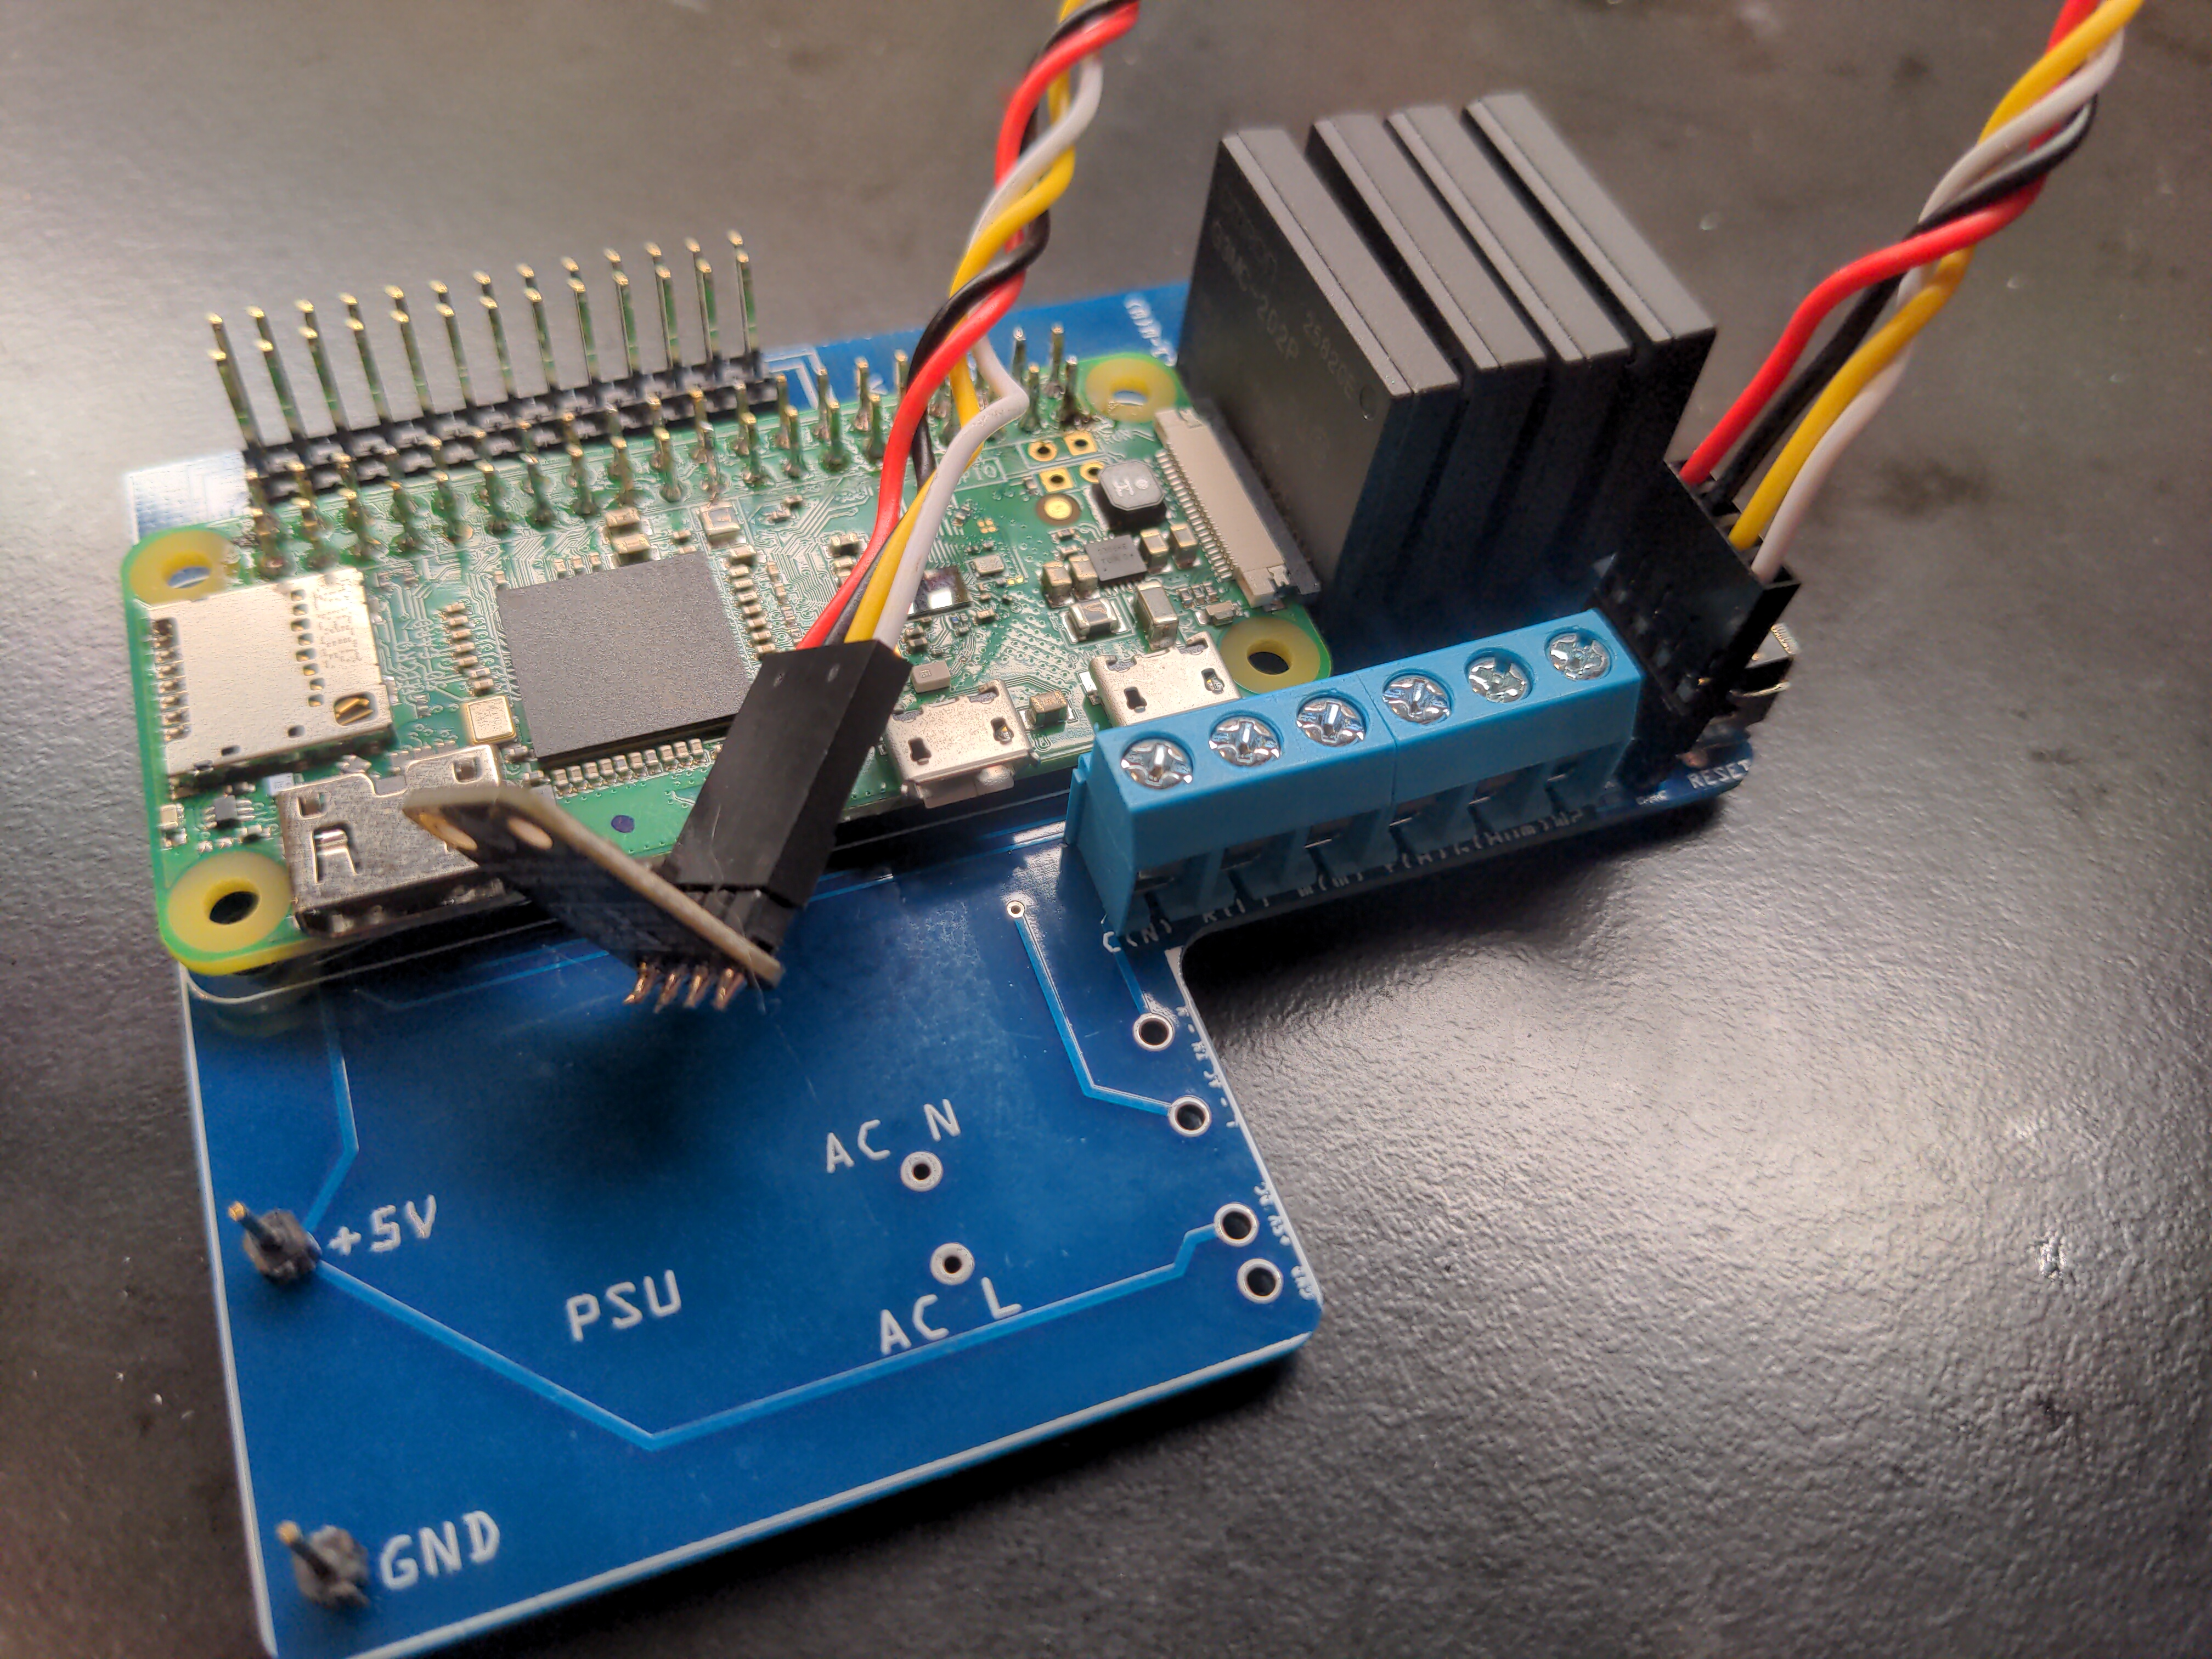
\includegraphics[width=3in]{img/fully_assembled.jpg}
  \caption{Fully assembled HestiaPi with headers for a DC power supply}
  \label{fig:fully_assembled}
\end{figure}

\subsubsection{Video}
\href{https://www.youtube.com/watch?v=gRcRINqT31g}{\includegraphics[width=5.0in]{img/hestiapi_one_soldering.jpg}}

\subsubsection{Hints and Tips}
The LCD needs to be connected before powering HestiaPi as it initialises on
boot only (otherwise it looks blank-white and touch events do not register) and
it may also cause a freeze or reboot due to power spike.

If you cannot control mains, that is having it off during all the time of
installation, our advise is to leave the SD card and LCD out, connect all
wires, partly (not fully) insert the SD and finish off case installation with
the LCD attached to the cover.

Once all is done, from outside of the case, push first the SD all the way in
(it does not lock-click in place) and then insert a non-metallic tool and press
the reset button from the right side. HestiaPi will boot and in about 10-15sec
the LCD will show some of the boot messages.

\subsubsection{Troubleshooting}
After assembling you HestiaPi, put in an SD card that has been flashed, attach
the touch screen and try booting it up.

If you get a blank screen, the pi might not be booting properly.  Make sure the
SD card was flashed properly.  A common mistake is to flash the image onto the
partition instead of the block device (e.g., /dev/sdb1 instead of /dev/sdb).

Test your reset button.  If it doesn't work, odds are it's either a faulty
component, or more likely a cold solder joint.  The former can be fixed by
replacing the part, and the latter by re-soldering the component onto the
board.  Use a multimeter to verify the switch works.  If it does, trace the
line to the pin on the pi to see if there is connectivity there.
